% CSE513 Assignment 1 report. Build: node scripts/report-data.mjs, then latexmk -pdf main.tex (in report/).
\documentclass[11pt,a4paper]{article}
\usepackage[margin=2.2cm]{geometry}
\usepackage[T1]{fontenc}
\usepackage{lmodern}
\usepackage{amssymb}
\usepackage{booktabs}
\usepackage{array}
\usepackage{graphicx}
\usepackage{tikz}
\usetikzlibrary{patterns}
\usepackage[hidelinks]{hyperref}
\usepackage{enumitem}
\setlist{itemsep=2pt, topsep=4pt}
\setlength{\parskip}{4pt}
\setlength{\parindent}{0pt}

\newcommand{\siteurl}{https://meliksahcaliskan.github.io/Scheduler_Simulation/}
\newcommand{\repourl}{https://github.com/Meliksahcaliskan/Scheduler_Simulation}
\newcommand{\authorname}{Meliksah Caliskan}
% Generated by scripts/report-data.mjs. Do not edit.
\newcommand{\stattests}{94}
\newcommand{\statpass}{90}
\newcommand{\statfail}{0}
\newcommand{\statskipped}{4}


\begin{document}

\begin{center}
  {\LARGE\bfseries CSE513 Assignment 1: CPU Scheduling Simulator}\\[6pt]
  {\large Website: \textcolor{blue}{\href{\siteurl}{\nolinkurl{\siteurl}}}}\\[6pt]
  \authorname\quad·\quad\today
\end{center}

\section{Overview and how to run}

The simulator is a single web page that schedules a set of processes with FCFS, SJF (non-preemptive),
SRTF (preemptive) or Round Robin with a configurable quantum. It shows a labeled Gantt chart (including idle
intervals and, for RR, every quantum slice as its own block), a results table with all seven per-process values and
the three averages, a verification panel that checks the five required properties on every run, a step-by-step player
that explains each scheduling decision, and a comparison of all four algorithms on the same input.

\begin{itemize}
  \item \textbf{Online:} \href{\siteurl}{\nolinkurl{\siteurl}} (GitHub Pages, no login needed).
  \item \textbf{Locally:} open \texttt{index.html} from the source archive by double-clicking it. It is one
    self-contained file (all JavaScript and CSS inline), so it needs no server, installation or network.
  \item \textbf{Source:} \href{\repourl}{\nolinkurl{\repourl}}. The \texttt{README.md} explains how to run, test and
    rebuild the page, the dependencies (none at runtime; Node.js only for the tests and the build) and the limitations.
\end{itemize}

\textbf{Model and rules.} One CPU; each process has one CPU burst and no I/O; context switches cost nothing; time is in
integer units and intervals are half-open ($[2,5)$ is 3 units). The CPU never idles while a process is ready.
FCFS picks the earliest arrival; SJF picks the shortest burst when the CPU becomes free; SRTF picks the shortest
remaining time and preempts only on a \emph{strictly} shorter remaining time. Ties go to the earlier arrival, then the
earlier row in the input. RR uses a FIFO queue; at a quantum boundary, processes arriving at that exact time are
enqueued before the preempted process, and a finished process never rejoins the queue.
Invalid input (empty or duplicate IDs, where \texttt{p1} and \texttt{P1} count as duplicates; non-integer or negative
times; zero bursts or quantum; values over the limits) is rejected with one message per problem, tied to its row and
marked on the field.

\textbf{Implementation.} The engine (\texttt{src/scheduler.js}) is a pure function that steps through time one unit
at a time. At every integer time $t$ it performs the same steps in a fixed order:
(1) complete the process that ran in $[t-1,t)$; (2) admit arrivals at $t$ in input order; (3) RR: expire the quantum and
re-enqueue the process \emph{after} the arrivals of step 2; (4) SRTF: preempt only if an arrival is strictly shorter;
(5) dispatch or start an idle interval; (6) run one unit. The RR boundary rule and ``finishing exactly at a boundary is a
completion, not an expiry'' follow from this order. Every decision is recorded as an event with a snapshot of the ready
queue; the step-by-step player shows these events, and a test checks that replaying them rebuilds the Gantt chart.

\begin{figure}[tb]
  \centering
  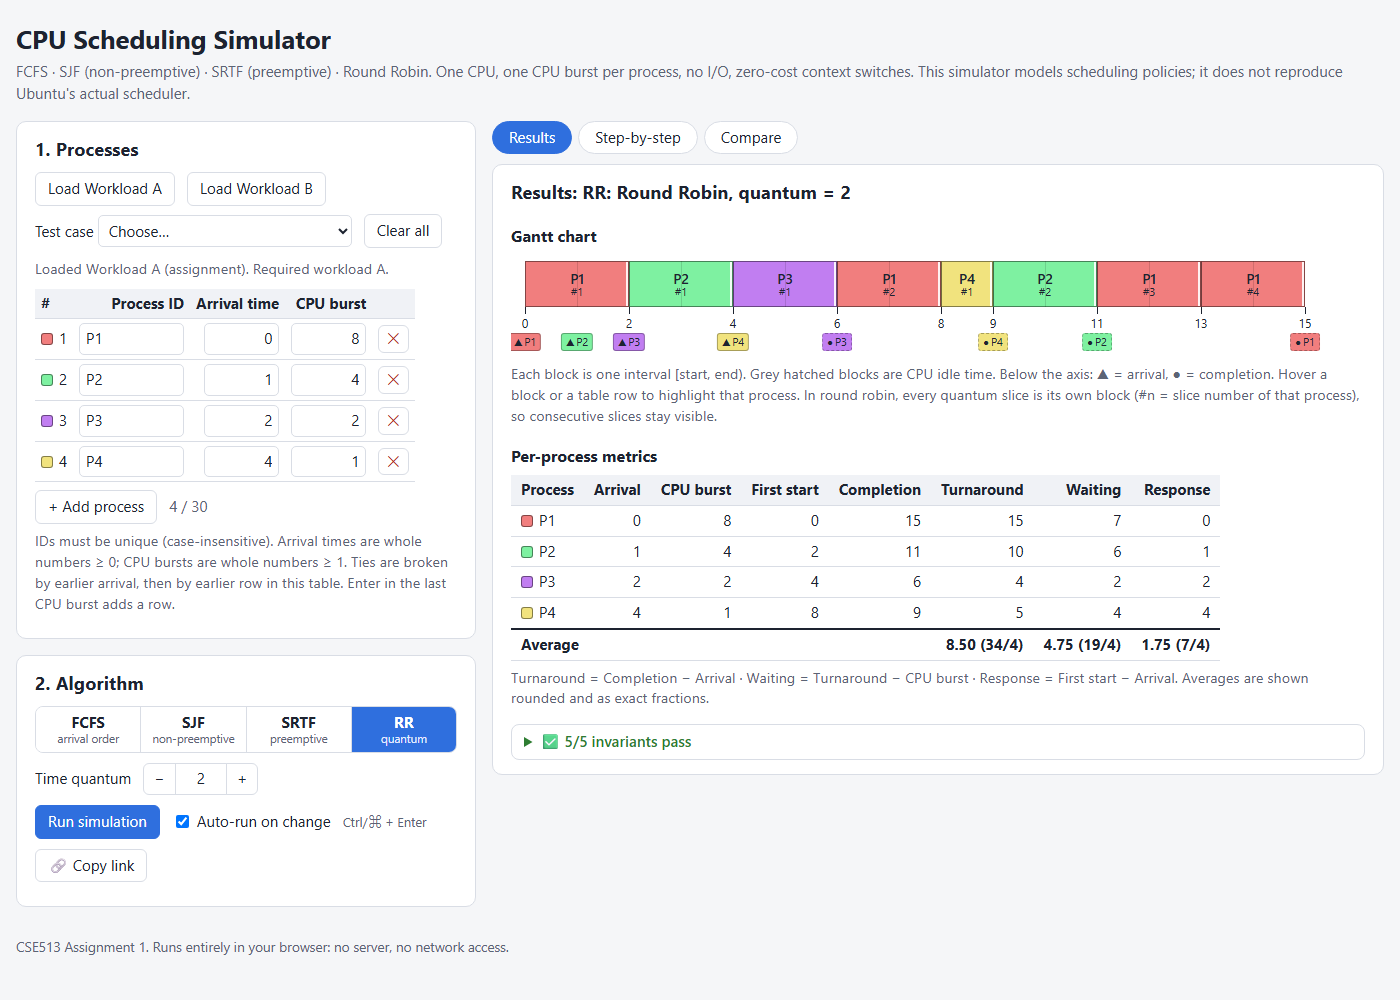
\includegraphics[width=0.85\textwidth]{figures/ui-results-A-RR.png}
  \caption{The website with Workload A, RR $q=2$: input on the left; Gantt chart with arrival (\(\blacktriangle\)) and
    completion (\(\bullet\)) markers, results table and verification badge on the right.}
\end{figure}

\section{Worked examples: Workloads A and B}

I calculated all eight timelines and metrics by hand on paper before checking them with the simulator
(scans in Appendix~\ref{app:hand}). The values were transcribed into \texttt{tests/oracle/hand.json}; an automated
test (\texttt{tests/oracle.test.js}) checks the arithmetic of the hand values and compares them with the simulator.
In each example below, the upper Gantt row is the hand timeline (from \texttt{hand.json}) and the lower row is the
simulator's output; in the tables, H = hand and S = simulator (a differing simulator value would be shown in red).
Start = first start time, Compl.\ = completion, TAT = turnaround, WT = waiting, RT = response.

\subsection{Workload A}
\begin{center}% Generated by scripts/report-data.mjs. Do not edit.
\begin{tabular}{lcc}
\toprule
Process & Arrival & CPU burst \\
\midrule
P1 & 0 & 8 \\
P2 & 1 & 4 \\
P3 & 2 & 2 \\
P4 & 4 & 1 \\
\bottomrule
\end{tabular}
\end{center}

\subsubsection*{A1. FCFS}
At $t=0$ only P1 is ready and runs to completion at 8 (non-preemptive). P2, P3 and P4 then run in arrival order.
The long first job delays every later one (convoy effect).
% Generated by scripts/report-data.mjs. Do not edit.
\par\noindent\begin{minipage}{\linewidth}
\begin{center}
\definecolor{pc-P1}{HTML}{F17E7E}
\definecolor{pc-P2}{HTML}{7EF1A1}
\definecolor{pc-P3}{HTML}{C17EF1}
\definecolor{pc-P4}{HTML}{F1E37E}
\begin{tikzpicture}[x=0.800cm, y=1cm, font=\footnotesize]
\node[anchor=east, font=\footnotesize\bfseries] at (-0.3/0.800, 0.3) {Hand};
\draw[fill=pc-P1, draw=black!70] (0, 0) rectangle (8, 0.6);
\node[align=center, inner sep=0pt] at (4, 0.3) {P1};
\draw[fill=pc-P2, draw=black!70] (8, 0) rectangle (12, 0.6);
\node[align=center, inner sep=0pt] at (10, 0.3) {P2};
\draw[fill=pc-P3, draw=black!70] (12, 0) rectangle (14, 0.6);
\node[align=center, inner sep=0pt] at (13, 0.3) {P3};
\draw[fill=pc-P4, draw=black!70] (14, 0) rectangle (15, 0.6);
\node[align=center, inner sep=0pt] at (14.5, 0.3) {P4};
\draw (0, 0) -- (0, -0.08) node[below, inner sep=1pt, font=\scriptsize] {0};
\draw (8, 0) -- (8, -0.08) node[below, inner sep=1pt, font=\scriptsize] {8};
\draw (12, 0) -- (12, -0.08) node[below, inner sep=1pt, font=\scriptsize] {12};
\draw (14, 0) -- (14, -0.08) node[below, inner sep=1pt, font=\scriptsize] {14};
\draw (15, 0) -- (15, -0.08) node[below, inner sep=1pt, font=\scriptsize] {15};
\node[anchor=east, font=\footnotesize\bfseries] at (-0.3/0.800, -0.85) {Simulator};
\draw[fill=pc-P1, draw=black!70] (0, -1.15) rectangle (8, -0.55);
\node[align=center, inner sep=0pt] at (4, -0.85) {P1};
\draw[fill=pc-P2, draw=black!70] (8, -1.15) rectangle (12, -0.55);
\node[align=center, inner sep=0pt] at (10, -0.85) {P2};
\draw[fill=pc-P3, draw=black!70] (12, -1.15) rectangle (14, -0.55);
\node[align=center, inner sep=0pt] at (13, -0.85) {P3};
\draw[fill=pc-P4, draw=black!70] (14, -1.15) rectangle (15, -0.55);
\node[align=center, inner sep=0pt] at (14.5, -0.85) {P4};
\draw (0, -1.15) -- (0, -1.23) node[below, inner sep=1pt, font=\scriptsize] {0};
\draw (8, -1.15) -- (8, -1.23) node[below, inner sep=1pt, font=\scriptsize] {8};
\draw (12, -1.15) -- (12, -1.23) node[below, inner sep=1pt, font=\scriptsize] {12};
\draw (14, -1.15) -- (14, -1.23) node[below, inner sep=1pt, font=\scriptsize] {14};
\draw (15, -1.15) -- (15, -1.23) node[below, inner sep=1pt, font=\scriptsize] {15};
\end{tikzpicture}
\end{center}
\begin{center}\small\setlength{\tabcolsep}{4pt}
\begin{tabular}{lcccccccccccc}
\toprule
 & & & \multicolumn{2}{c}{Start} & \multicolumn{2}{c}{Compl.} & \multicolumn{2}{c}{TAT} & \multicolumn{2}{c}{WT} & \multicolumn{2}{c}{RT} \\
\cmidrule(lr){4-5} \cmidrule(lr){6-7} \cmidrule(lr){8-9} \cmidrule(lr){10-11} \cmidrule(lr){12-13}
Proc. & Arr. & Burst & H & S & H & S & H & S & H & S & H & S \\
\midrule
P1 & 0 & 8 & 0 & 0 & 8 & 8 & 8 & 8 & 0 & 0 & 0 & 0 \\
P2 & 1 & 4 & 8 & 8 & 12 & 12 & 11 & 11 & 7 & 7 & 7 & 7 \\
P3 & 2 & 2 & 12 & 12 & 14 & 14 & 12 & 12 & 10 & 10 & 10 & 10 \\
P4 & 4 & 1 & 14 & 14 & 15 & 15 & 11 & 11 & 10 & 10 & 10 & 10 \\
\midrule
\multicolumn{7}{l}{Average (exact fractions)} & \multicolumn{2}{c}{42/4} & \multicolumn{2}{c}{27/4} & \multicolumn{2}{c}{27/4} \\
\bottomrule
\end{tabular}
\end{center}
\noindent\textbf{Comparison.} Hand (H) and simulator (S) agree on all 4 Gantt segments, all 20 per-process values and the 3 averages (turnaround 10.50 (42/4), waiting 6.75 (27/4), response 6.75 (27/4)). No discrepancy. The simulator's 5 invariants: 5/5 pass.
\end{minipage}\par\medskip


\subsubsection*{A2. SJF (non-preemptive)}
P1 is alone at $t=0$ and keeps the CPU until 8. At 8 the ready bursts are P2 = 4, P3 = 2, P4 = 1, so P4 runs, then
P3 (2 $<$ 4), then P2.
% Generated by scripts/report-data.mjs. Do not edit.
\par\noindent\begin{minipage}{\linewidth}
\begin{center}
\definecolor{pc-P1}{HTML}{F17E7E}
\definecolor{pc-P2}{HTML}{7EF1A1}
\definecolor{pc-P3}{HTML}{C17EF1}
\definecolor{pc-P4}{HTML}{F1E37E}
\begin{tikzpicture}[x=0.800cm, y=1cm, font=\footnotesize]
\node[anchor=east, font=\footnotesize\bfseries] at (-0.3/0.800, 0.3) {Hand};
\draw[fill=pc-P1, draw=black!70] (0, 0) rectangle (8, 0.6);
\node[align=center, inner sep=0pt] at (4, 0.3) {P1};
\draw[fill=pc-P4, draw=black!70] (8, 0) rectangle (9, 0.6);
\node[align=center, inner sep=0pt] at (8.5, 0.3) {P4};
\draw[fill=pc-P3, draw=black!70] (9, 0) rectangle (11, 0.6);
\node[align=center, inner sep=0pt] at (10, 0.3) {P3};
\draw[fill=pc-P2, draw=black!70] (11, 0) rectangle (15, 0.6);
\node[align=center, inner sep=0pt] at (13, 0.3) {P2};
\draw (0, 0) -- (0, -0.08) node[below, inner sep=1pt, font=\scriptsize] {0};
\draw (8, 0) -- (8, -0.08) node[below, inner sep=1pt, font=\scriptsize] {8};
\draw (9, 0) -- (9, -0.08) node[below, inner sep=1pt, font=\scriptsize] {9};
\draw (11, 0) -- (11, -0.08) node[below, inner sep=1pt, font=\scriptsize] {11};
\draw (15, 0) -- (15, -0.08) node[below, inner sep=1pt, font=\scriptsize] {15};
\node[anchor=east, font=\footnotesize\bfseries] at (-0.3/0.800, -0.8499999999999999) {Simulator};
\draw[fill=pc-P1, draw=black!70] (0, -1.15) rectangle (8, -0.5499999999999999);
\node[align=center, inner sep=0pt] at (4, -0.8499999999999999) {P1};
\draw[fill=pc-P4, draw=black!70] (8, -1.15) rectangle (9, -0.5499999999999999);
\node[align=center, inner sep=0pt] at (8.5, -0.8499999999999999) {P4};
\draw[fill=pc-P3, draw=black!70] (9, -1.15) rectangle (11, -0.5499999999999999);
\node[align=center, inner sep=0pt] at (10, -0.8499999999999999) {P3};
\draw[fill=pc-P2, draw=black!70] (11, -1.15) rectangle (15, -0.5499999999999999);
\node[align=center, inner sep=0pt] at (13, -0.8499999999999999) {P2};
\draw (0, -1.15) -- (0, -1.23) node[below, inner sep=1pt, font=\scriptsize] {0};
\draw (8, -1.15) -- (8, -1.23) node[below, inner sep=1pt, font=\scriptsize] {8};
\draw (9, -1.15) -- (9, -1.23) node[below, inner sep=1pt, font=\scriptsize] {9};
\draw (11, -1.15) -- (11, -1.23) node[below, inner sep=1pt, font=\scriptsize] {11};
\draw (15, -1.15) -- (15, -1.23) node[below, inner sep=1pt, font=\scriptsize] {15};
\end{tikzpicture}
\end{center}
\begin{center}\small\setlength{\tabcolsep}{4pt}
\begin{tabular}{lcccccccccccc}
\toprule
 & & & \multicolumn{2}{c}{Start} & \multicolumn{2}{c}{Compl.} & \multicolumn{2}{c}{TAT} & \multicolumn{2}{c}{WT} & \multicolumn{2}{c}{RT} \\
\cmidrule(lr){4-5} \cmidrule(lr){6-7} \cmidrule(lr){8-9} \cmidrule(lr){10-11} \cmidrule(lr){12-13}
Proc. & Arr. & Burst & H & S & H & S & H & S & H & S & H & S \\
\midrule
P1 & 0 & 8 & 0 & 0 & 8 & 8 & 8 & 8 & 0 & 0 & 0 & 0 \\
P2 & 1 & 4 & 11 & 11 & 15 & 15 & 14 & 14 & 10 & 10 & 10 & 10 \\
P3 & 2 & 2 & 9 & 9 & 11 & 11 & 9 & 9 & 7 & 7 & 7 & 7 \\
P4 & 4 & 1 & 8 & 8 & 9 & 9 & 5 & 5 & 4 & 4 & 4 & 4 \\
\midrule
\multicolumn{7}{l}{Average (exact fractions)} & \multicolumn{2}{c}{36/4} & \multicolumn{2}{c}{21/4} & \multicolumn{2}{c}{21/4} \\
\bottomrule
\end{tabular}
\end{center}
\noindent\textbf{Comparison.} Hand (H) and simulator (S) agree on all 4 Gantt segments, all 20 per-process values and the 3 averages (turnaround 9.00 (36/4), waiting 5.25 (21/4), response 5.25 (21/4)). No discrepancy. The simulator's 5 invariants: 5/5 pass.
\end{minipage}\par\medskip


\subsubsection*{A3. SRTF (preemptive)}
$t=1$: P2 arrives with 4 $<$ P1's remaining 7, so P1 is preempted. $t=2$: P3 (2) $<$ P2's remaining 3, so P2 is
preempted. $t=4$: P3 completes and P4 arrives; P4 (1) is the shortest of P4, P2 (3), P1 (7). P2 then finishes at 8 and
P1 at 15. Every process starts the moment it arrives.
% Generated by scripts/report-data.mjs. Do not edit.
\par\noindent\begin{minipage}{\linewidth}
\begin{center}
\definecolor{pc-P1}{HTML}{F17E7E}
\definecolor{pc-P2}{HTML}{7EF1A1}
\definecolor{pc-P3}{HTML}{C17EF1}
\definecolor{pc-P4}{HTML}{F1E37E}
\begin{tikzpicture}[x=0.800cm, y=1cm, font=\footnotesize]
\node[anchor=east, font=\footnotesize\bfseries] at (-0.3/0.800, 0.3) {Hand};
\draw[fill=pc-P1, draw=black!70] (0, 0) rectangle (1, 0.6);
\node[align=center, inner sep=0pt] at (0.5, 0.3) {P1};
\draw[fill=pc-P2, draw=black!70] (1, 0) rectangle (2, 0.6);
\node[align=center, inner sep=0pt] at (1.5, 0.3) {P2};
\draw[fill=pc-P3, draw=black!70] (2, 0) rectangle (4, 0.6);
\node[align=center, inner sep=0pt] at (3, 0.3) {P3};
\draw[fill=pc-P4, draw=black!70] (4, 0) rectangle (5, 0.6);
\node[align=center, inner sep=0pt] at (4.5, 0.3) {P4};
\draw[fill=pc-P2, draw=black!70] (5, 0) rectangle (8, 0.6);
\node[align=center, inner sep=0pt] at (6.5, 0.3) {P2};
\draw[fill=pc-P1, draw=black!70] (8, 0) rectangle (15, 0.6);
\node[align=center, inner sep=0pt] at (11.5, 0.3) {P1};
\draw (0, 0) -- (0, -0.08) node[below, inner sep=1pt, font=\scriptsize] {0};
\draw (1, 0) -- (1, -0.08) node[below, inner sep=1pt, font=\scriptsize] {1};
\draw (2, 0) -- (2, -0.08) node[below, inner sep=1pt, font=\scriptsize] {2};
\draw (4, 0) -- (4, -0.08) node[below, inner sep=1pt, font=\scriptsize] {4};
\draw (5, 0) -- (5, -0.08) node[below, inner sep=1pt, font=\scriptsize] {5};
\draw (8, 0) -- (8, -0.08) node[below, inner sep=1pt, font=\scriptsize] {8};
\draw (15, 0) -- (15, -0.08) node[below, inner sep=1pt, font=\scriptsize] {15};
\node[anchor=east, font=\footnotesize\bfseries] at (-0.3/0.800, -0.85) {Simulator};
\draw[fill=pc-P1, draw=black!70] (0, -1.15) rectangle (1, -0.55);
\node[align=center, inner sep=0pt] at (0.5, -0.85) {P1};
\draw[fill=pc-P2, draw=black!70] (1, -1.15) rectangle (2, -0.55);
\node[align=center, inner sep=0pt] at (1.5, -0.85) {P2};
\draw[fill=pc-P3, draw=black!70] (2, -1.15) rectangle (4, -0.55);
\node[align=center, inner sep=0pt] at (3, -0.85) {P3};
\draw[fill=pc-P4, draw=black!70] (4, -1.15) rectangle (5, -0.55);
\node[align=center, inner sep=0pt] at (4.5, -0.85) {P4};
\draw[fill=pc-P2, draw=black!70] (5, -1.15) rectangle (8, -0.55);
\node[align=center, inner sep=0pt] at (6.5, -0.85) {P2};
\draw[fill=pc-P1, draw=black!70] (8, -1.15) rectangle (15, -0.55);
\node[align=center, inner sep=0pt] at (11.5, -0.85) {P1};
\draw (0, -1.15) -- (0, -1.23) node[below, inner sep=1pt, font=\scriptsize] {0};
\draw (1, -1.15) -- (1, -1.23) node[below, inner sep=1pt, font=\scriptsize] {1};
\draw (2, -1.15) -- (2, -1.23) node[below, inner sep=1pt, font=\scriptsize] {2};
\draw (4, -1.15) -- (4, -1.23) node[below, inner sep=1pt, font=\scriptsize] {4};
\draw (5, -1.15) -- (5, -1.23) node[below, inner sep=1pt, font=\scriptsize] {5};
\draw (8, -1.15) -- (8, -1.23) node[below, inner sep=1pt, font=\scriptsize] {8};
\draw (15, -1.15) -- (15, -1.23) node[below, inner sep=1pt, font=\scriptsize] {15};
\end{tikzpicture}
\end{center}
\begin{center}\small\setlength{\tabcolsep}{4pt}
\begin{tabular}{lcccccccccccc}
\toprule
 & & & \multicolumn{2}{c}{Start} & \multicolumn{2}{c}{Compl.} & \multicolumn{2}{c}{TAT} & \multicolumn{2}{c}{WT} & \multicolumn{2}{c}{RT} \\
\cmidrule(lr){4-5} \cmidrule(lr){6-7} \cmidrule(lr){8-9} \cmidrule(lr){10-11} \cmidrule(lr){12-13}
Proc. & Arr. & Burst & H & S & H & S & H & S & H & S & H & S \\
\midrule
P1 & 0 & 8 & 0 & 0 & 15 & 15 & 15 & 15 & 7 & 7 & 0 & 0 \\
P2 & 1 & 4 & 1 & 1 & 8 & 8 & 7 & 7 & 3 & 3 & 0 & 0 \\
P3 & 2 & 2 & 2 & 2 & 4 & 4 & 2 & 2 & 0 & 0 & 0 & 0 \\
P4 & 4 & 1 & 4 & 4 & 5 & 5 & 1 & 1 & 0 & 0 & 0 & 0 \\
\midrule
\multicolumn{7}{l}{Average (exact fractions)} & \multicolumn{2}{c}{25/4} & \multicolumn{2}{c}{10/4} & \multicolumn{2}{c}{0/4} \\
\bottomrule
\end{tabular}
\end{center}
\noindent\textbf{Comparison.} Hand (H) and simulator (S) agree on all 6 Gantt segments, all 20 per-process values and the 3 averages (turnaround 6.25 (25/4), waiting 2.50 (10/4), response 0.00 (0/4)). No discrepancy. The simulator's 5 invariants: 5/5 pass.
\end{minipage}\par\medskip


\subsubsection*{A4. Round Robin, $q=2$}
P1 runs $[0,2)$. At $t=2$, P3 arrives exactly at the boundary, so the queue is P2, P3, P1 (P3 before the preempted P1).
At $t=4$, P4 arrives at P2's boundary: queue P3, P1, P4, P2. P3 and P4 finish inside their slices; P1 needs four slices,
and the last two are consecutive (\#3, \#4) because it is then alone. The chart keeps them as two blocks.
% Generated by scripts/report-data.mjs. Do not edit.
\par\noindent\begin{minipage}{\linewidth}
\begin{center}
\definecolor{pc-P1}{HTML}{F17E7E}
\definecolor{pc-P2}{HTML}{7EF1A1}
\definecolor{pc-P3}{HTML}{C17EF1}
\definecolor{pc-P4}{HTML}{F1E37E}
\begin{tikzpicture}[x=0.800cm, y=1cm, font=\footnotesize]
\node[anchor=east, font=\footnotesize\bfseries] at (-0.3/0.800, 0.3) {Hand};
\draw[fill=pc-P1, draw=black!70] (0, 0) rectangle (2, 0.6);
\node[align=center, inner sep=0pt] at (1, 0.3) {P1\\[-2pt]{\tiny\#1}};
\draw[fill=pc-P2, draw=black!70] (2, 0) rectangle (4, 0.6);
\node[align=center, inner sep=0pt] at (3, 0.3) {P2\\[-2pt]{\tiny\#1}};
\draw[fill=pc-P3, draw=black!70] (4, 0) rectangle (6, 0.6);
\node[align=center, inner sep=0pt] at (5, 0.3) {P3\\[-2pt]{\tiny\#1}};
\draw[fill=pc-P1, draw=black!70] (6, 0) rectangle (8, 0.6);
\node[align=center, inner sep=0pt] at (7, 0.3) {P1\\[-2pt]{\tiny\#2}};
\draw[fill=pc-P4, draw=black!70] (8, 0) rectangle (9, 0.6);
\node[align=center, inner sep=0pt] at (8.5, 0.3) {P4\\[-2pt]{\tiny\#1}};
\draw[fill=pc-P2, draw=black!70] (9, 0) rectangle (11, 0.6);
\node[align=center, inner sep=0pt] at (10, 0.3) {P2\\[-2pt]{\tiny\#2}};
\draw[fill=pc-P1, draw=black!70] (11, 0) rectangle (13, 0.6);
\node[align=center, inner sep=0pt] at (12, 0.3) {P1\\[-2pt]{\tiny\#3}};
\draw[fill=pc-P1, draw=black!70] (13, 0) rectangle (15, 0.6);
\node[align=center, inner sep=0pt] at (14, 0.3) {P1\\[-2pt]{\tiny\#4}};
\draw (0, 0) -- (0, -0.08) node[below, inner sep=1pt, font=\scriptsize] {0};
\draw (2, 0) -- (2, -0.08) node[below, inner sep=1pt, font=\scriptsize] {2};
\draw (4, 0) -- (4, -0.08) node[below, inner sep=1pt, font=\scriptsize] {4};
\draw (6, 0) -- (6, -0.08) node[below, inner sep=1pt, font=\scriptsize] {6};
\draw (8, 0) -- (8, -0.08) node[below, inner sep=1pt, font=\scriptsize] {8};
\draw (9, 0) -- (9, -0.08) node[below, inner sep=1pt, font=\scriptsize] {9};
\draw (11, 0) -- (11, -0.08) node[below, inner sep=1pt, font=\scriptsize] {11};
\draw (13, 0) -- (13, -0.08) node[below, inner sep=1pt, font=\scriptsize] {13};
\draw (15, 0) -- (15, -0.08) node[below, inner sep=1pt, font=\scriptsize] {15};
\node[anchor=east, font=\footnotesize\bfseries] at (-0.3/0.800, -0.85) {Simulator};
\draw[fill=pc-P1, draw=black!70] (0, -1.15) rectangle (2, -0.55);
\node[align=center, inner sep=0pt] at (1, -0.85) {P1\\[-2pt]{\tiny\#1}};
\draw[fill=pc-P2, draw=black!70] (2, -1.15) rectangle (4, -0.55);
\node[align=center, inner sep=0pt] at (3, -0.85) {P2\\[-2pt]{\tiny\#1}};
\draw[fill=pc-P3, draw=black!70] (4, -1.15) rectangle (6, -0.55);
\node[align=center, inner sep=0pt] at (5, -0.85) {P3\\[-2pt]{\tiny\#1}};
\draw[fill=pc-P1, draw=black!70] (6, -1.15) rectangle (8, -0.55);
\node[align=center, inner sep=0pt] at (7, -0.85) {P1\\[-2pt]{\tiny\#2}};
\draw[fill=pc-P4, draw=black!70] (8, -1.15) rectangle (9, -0.55);
\node[align=center, inner sep=0pt] at (8.5, -0.85) {P4\\[-2pt]{\tiny\#1}};
\draw[fill=pc-P2, draw=black!70] (9, -1.15) rectangle (11, -0.55);
\node[align=center, inner sep=0pt] at (10, -0.85) {P2\\[-2pt]{\tiny\#2}};
\draw[fill=pc-P1, draw=black!70] (11, -1.15) rectangle (13, -0.55);
\node[align=center, inner sep=0pt] at (12, -0.85) {P1\\[-2pt]{\tiny\#3}};
\draw[fill=pc-P1, draw=black!70] (13, -1.15) rectangle (15, -0.55);
\node[align=center, inner sep=0pt] at (14, -0.85) {P1\\[-2pt]{\tiny\#4}};
\draw (0, -1.15) -- (0, -1.23) node[below, inner sep=1pt, font=\scriptsize] {0};
\draw (2, -1.15) -- (2, -1.23) node[below, inner sep=1pt, font=\scriptsize] {2};
\draw (4, -1.15) -- (4, -1.23) node[below, inner sep=1pt, font=\scriptsize] {4};
\draw (6, -1.15) -- (6, -1.23) node[below, inner sep=1pt, font=\scriptsize] {6};
\draw (8, -1.15) -- (8, -1.23) node[below, inner sep=1pt, font=\scriptsize] {8};
\draw (9, -1.15) -- (9, -1.23) node[below, inner sep=1pt, font=\scriptsize] {9};
\draw (11, -1.15) -- (11, -1.23) node[below, inner sep=1pt, font=\scriptsize] {11};
\draw (13, -1.15) -- (13, -1.23) node[below, inner sep=1pt, font=\scriptsize] {13};
\draw (15, -1.15) -- (15, -1.23) node[below, inner sep=1pt, font=\scriptsize] {15};
\end{tikzpicture}
\end{center}
\begin{center}\small\setlength{\tabcolsep}{4pt}
\begin{tabular}{lcccccccccccc}
\toprule
 & & & \multicolumn{2}{c}{Start} & \multicolumn{2}{c}{Compl.} & \multicolumn{2}{c}{TAT} & \multicolumn{2}{c}{WT} & \multicolumn{2}{c}{RT} \\
\cmidrule(lr){4-5} \cmidrule(lr){6-7} \cmidrule(lr){8-9} \cmidrule(lr){10-11} \cmidrule(lr){12-13}
Proc. & Arr. & Burst & H & S & H & S & H & S & H & S & H & S \\
\midrule
P1 & 0 & 8 & 0 & 0 & 15 & 15 & 15 & 15 & 7 & 7 & 0 & 0 \\
P2 & 1 & 4 & 2 & 2 & 11 & 11 & 10 & 10 & 6 & 6 & 1 & 1 \\
P3 & 2 & 2 & 4 & 4 & 6 & 6 & 4 & 4 & 2 & 2 & 2 & 2 \\
P4 & 4 & 1 & 8 & 8 & 9 & 9 & 5 & 5 & 4 & 4 & 4 & 4 \\
\midrule
\multicolumn{7}{l}{Average (exact fractions)} & \multicolumn{2}{c}{34/4} & \multicolumn{2}{c}{19/4} & \multicolumn{2}{c}{7/4} \\
\bottomrule
\end{tabular}
\end{center}
\noindent\textbf{Comparison.} Hand (H) and simulator (S) agree on all 8 Gantt segments, all 20 per-process values and the 3 averages (turnaround 8.50 (34/4), waiting 4.75 (19/4), response 1.75 (7/4)). No discrepancy. The simulator's 5 invariants: 5/5 pass.
\end{minipage}\par\medskip


\subsection{Workload B}
\begin{center}% Generated by scripts/report-data.mjs. Do not edit.
\begin{tabular}{lcc}
\toprule
Process & Arrival & CPU burst \\
\midrule
P1 & 2 & 3 \\
P2 & 2 & 1 \\
P3 & 8 & 2 \\
P4 & 9 & 1 \\
\bottomrule
\end{tabular}
\end{center}
(My handwritten page for B is titled ``Workload A'' by mistake; its process table and all values are Workload B's.)

\subsubsection*{B1. FCFS}
The CPU is idle until the first arrival at $t=2$. P1 and P2 arrive together, so the tie is broken by input order: P1
first. The CPU idles again in $[6,8)$; P4 arrives at 9 while P3 runs and waits until 10.
% Generated by scripts/report-data.mjs. Do not edit.
\par\noindent\begin{minipage}{\linewidth}
\begin{center}
\definecolor{pc-P1}{HTML}{F17E7E}
\definecolor{pc-P2}{HTML}{7EF1A1}
\definecolor{pc-P3}{HTML}{C17EF1}
\definecolor{pc-P4}{HTML}{F1E37E}
\begin{tikzpicture}[x=0.800cm, y=1cm, font=\footnotesize]
\node[anchor=east, font=\footnotesize\bfseries] at (-0.3/0.800, 0.3) {Hand};
\draw[pattern=north east lines, pattern color=black!35, draw=black!70] (0, 0) rectangle (2, 0.6);
\node[align=center, inner sep=0pt] at (1, 0.3) {\textit{idle}};
\draw[fill=pc-P1, draw=black!70] (2, 0) rectangle (5, 0.6);
\node[align=center, inner sep=0pt] at (3.5, 0.3) {P1};
\draw[fill=pc-P2, draw=black!70] (5, 0) rectangle (6, 0.6);
\node[align=center, inner sep=0pt] at (5.5, 0.3) {P2};
\draw[pattern=north east lines, pattern color=black!35, draw=black!70] (6, 0) rectangle (8, 0.6);
\node[align=center, inner sep=0pt] at (7, 0.3) {\textit{idle}};
\draw[fill=pc-P3, draw=black!70] (8, 0) rectangle (10, 0.6);
\node[align=center, inner sep=0pt] at (9, 0.3) {P3};
\draw[fill=pc-P4, draw=black!70] (10, 0) rectangle (11, 0.6);
\node[align=center, inner sep=0pt] at (10.5, 0.3) {P4};
\draw (0, 0) -- (0, -0.08) node[below, inner sep=1pt, font=\scriptsize] {0};
\draw (2, 0) -- (2, -0.08) node[below, inner sep=1pt, font=\scriptsize] {2};
\draw (5, 0) -- (5, -0.08) node[below, inner sep=1pt, font=\scriptsize] {5};
\draw (6, 0) -- (6, -0.08) node[below, inner sep=1pt, font=\scriptsize] {6};
\draw (8, 0) -- (8, -0.08) node[below, inner sep=1pt, font=\scriptsize] {8};
\draw (10, 0) -- (10, -0.08) node[below, inner sep=1pt, font=\scriptsize] {10};
\draw (11, 0) -- (11, -0.08) node[below, inner sep=1pt, font=\scriptsize] {11};
\node[anchor=east, font=\footnotesize\bfseries] at (-0.3/0.800, -0.8499999999999999) {Simulator};
\draw[pattern=north east lines, pattern color=black!35, draw=black!70] (0, -1.15) rectangle (2, -0.5499999999999999);
\node[align=center, inner sep=0pt] at (1, -0.8499999999999999) {\textit{idle}};
\draw[fill=pc-P1, draw=black!70] (2, -1.15) rectangle (5, -0.5499999999999999);
\node[align=center, inner sep=0pt] at (3.5, -0.8499999999999999) {P1};
\draw[fill=pc-P2, draw=black!70] (5, -1.15) rectangle (6, -0.5499999999999999);
\node[align=center, inner sep=0pt] at (5.5, -0.8499999999999999) {P2};
\draw[pattern=north east lines, pattern color=black!35, draw=black!70] (6, -1.15) rectangle (8, -0.5499999999999999);
\node[align=center, inner sep=0pt] at (7, -0.8499999999999999) {\textit{idle}};
\draw[fill=pc-P3, draw=black!70] (8, -1.15) rectangle (10, -0.5499999999999999);
\node[align=center, inner sep=0pt] at (9, -0.8499999999999999) {P3};
\draw[fill=pc-P4, draw=black!70] (10, -1.15) rectangle (11, -0.5499999999999999);
\node[align=center, inner sep=0pt] at (10.5, -0.8499999999999999) {P4};
\draw (0, -1.15) -- (0, -1.23) node[below, inner sep=1pt, font=\scriptsize] {0};
\draw (2, -1.15) -- (2, -1.23) node[below, inner sep=1pt, font=\scriptsize] {2};
\draw (5, -1.15) -- (5, -1.23) node[below, inner sep=1pt, font=\scriptsize] {5};
\draw (6, -1.15) -- (6, -1.23) node[below, inner sep=1pt, font=\scriptsize] {6};
\draw (8, -1.15) -- (8, -1.23) node[below, inner sep=1pt, font=\scriptsize] {8};
\draw (10, -1.15) -- (10, -1.23) node[below, inner sep=1pt, font=\scriptsize] {10};
\draw (11, -1.15) -- (11, -1.23) node[below, inner sep=1pt, font=\scriptsize] {11};
\end{tikzpicture}
\end{center}
\begin{center}\small\setlength{\tabcolsep}{4pt}
\begin{tabular}{lcccccccccccc}
\toprule
 & & & \multicolumn{2}{c}{Start} & \multicolumn{2}{c}{Compl.} & \multicolumn{2}{c}{TAT} & \multicolumn{2}{c}{WT} & \multicolumn{2}{c}{RT} \\
\cmidrule(lr){4-5} \cmidrule(lr){6-7} \cmidrule(lr){8-9} \cmidrule(lr){10-11} \cmidrule(lr){12-13}
Proc. & Arr. & Burst & H & S & H & S & H & S & H & S & H & S \\
\midrule
P1 & 2 & 3 & 2 & 2 & 5 & 5 & 3 & 3 & 0 & 0 & 0 & 0 \\
P2 & 2 & 1 & 5 & 5 & 6 & 6 & 4 & 4 & 3 & 3 & 3 & 3 \\
P3 & 8 & 2 & 8 & 8 & 10 & 10 & 2 & 2 & 0 & 0 & 0 & 0 \\
P4 & 9 & 1 & 10 & 10 & 11 & 11 & 2 & 2 & 1 & 1 & 1 & 1 \\
\midrule
\multicolumn{7}{l}{Average (exact fractions)} & \multicolumn{2}{c}{11/4} & \multicolumn{2}{c}{4/4} & \multicolumn{2}{c}{4/4} \\
\bottomrule
\end{tabular}
\end{center}
\noindent\textbf{Comparison.} Hand (H) and simulator (S) agree on all 6 Gantt segments, all 20 per-process values and the 3 averages (turnaround 2.75 (11/4), waiting 1.00 (4/4), response 1.00 (4/4)). No discrepancy. The simulator's 5 invariants: 5/5 pass.
\end{minipage}\par\medskip


\subsubsection*{B2. SJF (non-preemptive)}
At $t=2$ P2 (burst 1) is shorter than P1 (3) and runs first. At 9, P4 arrives while P3 runs; SJF does not preempt, so P4
waits until 10.
% Generated by scripts/report-data.mjs. Do not edit.
\par\noindent\begin{minipage}{\linewidth}
\begin{center}
\definecolor{pc-P1}{HTML}{F17E7E}
\definecolor{pc-P2}{HTML}{7EF1A1}
\definecolor{pc-P3}{HTML}{C17EF1}
\definecolor{pc-P4}{HTML}{F1E37E}
\begin{tikzpicture}[x=0.800cm, y=1cm, font=\footnotesize]
\node[anchor=east, font=\footnotesize\bfseries] at (-0.3/0.800, 0.3) {Hand};
\draw[pattern=north east lines, pattern color=black!35, draw=black!70] (0, 0) rectangle (2, 0.6);
\node[align=center, inner sep=0pt] at (1, 0.3) {\textit{idle}};
\draw[fill=pc-P2, draw=black!70] (2, 0) rectangle (3, 0.6);
\node[align=center, inner sep=0pt] at (2.5, 0.3) {P2};
\draw[fill=pc-P1, draw=black!70] (3, 0) rectangle (6, 0.6);
\node[align=center, inner sep=0pt] at (4.5, 0.3) {P1};
\draw[pattern=north east lines, pattern color=black!35, draw=black!70] (6, 0) rectangle (8, 0.6);
\node[align=center, inner sep=0pt] at (7, 0.3) {\textit{idle}};
\draw[fill=pc-P3, draw=black!70] (8, 0) rectangle (10, 0.6);
\node[align=center, inner sep=0pt] at (9, 0.3) {P3};
\draw[fill=pc-P4, draw=black!70] (10, 0) rectangle (11, 0.6);
\node[align=center, inner sep=0pt] at (10.5, 0.3) {P4};
\draw (0, 0) -- (0, -0.08) node[below, inner sep=1pt, font=\scriptsize] {0};
\draw (2, 0) -- (2, -0.08) node[below, inner sep=1pt, font=\scriptsize] {2};
\draw (3, 0) -- (3, -0.08) node[below, inner sep=1pt, font=\scriptsize] {3};
\draw (6, 0) -- (6, -0.08) node[below, inner sep=1pt, font=\scriptsize] {6};
\draw (8, 0) -- (8, -0.08) node[below, inner sep=1pt, font=\scriptsize] {8};
\draw (10, 0) -- (10, -0.08) node[below, inner sep=1pt, font=\scriptsize] {10};
\draw (11, 0) -- (11, -0.08) node[below, inner sep=1pt, font=\scriptsize] {11};
\node[anchor=east, font=\footnotesize\bfseries] at (-0.3/0.800, -0.85) {Simulator};
\draw[pattern=north east lines, pattern color=black!35, draw=black!70] (0, -1.15) rectangle (2, -0.55);
\node[align=center, inner sep=0pt] at (1, -0.85) {\textit{idle}};
\draw[fill=pc-P2, draw=black!70] (2, -1.15) rectangle (3, -0.55);
\node[align=center, inner sep=0pt] at (2.5, -0.85) {P2};
\draw[fill=pc-P1, draw=black!70] (3, -1.15) rectangle (6, -0.55);
\node[align=center, inner sep=0pt] at (4.5, -0.85) {P1};
\draw[pattern=north east lines, pattern color=black!35, draw=black!70] (6, -1.15) rectangle (8, -0.55);
\node[align=center, inner sep=0pt] at (7, -0.85) {\textit{idle}};
\draw[fill=pc-P3, draw=black!70] (8, -1.15) rectangle (10, -0.55);
\node[align=center, inner sep=0pt] at (9, -0.85) {P3};
\draw[fill=pc-P4, draw=black!70] (10, -1.15) rectangle (11, -0.55);
\node[align=center, inner sep=0pt] at (10.5, -0.85) {P4};
\draw (0, -1.15) -- (0, -1.23) node[below, inner sep=1pt, font=\scriptsize] {0};
\draw (2, -1.15) -- (2, -1.23) node[below, inner sep=1pt, font=\scriptsize] {2};
\draw (3, -1.15) -- (3, -1.23) node[below, inner sep=1pt, font=\scriptsize] {3};
\draw (6, -1.15) -- (6, -1.23) node[below, inner sep=1pt, font=\scriptsize] {6};
\draw (8, -1.15) -- (8, -1.23) node[below, inner sep=1pt, font=\scriptsize] {8};
\draw (10, -1.15) -- (10, -1.23) node[below, inner sep=1pt, font=\scriptsize] {10};
\draw (11, -1.15) -- (11, -1.23) node[below, inner sep=1pt, font=\scriptsize] {11};
\end{tikzpicture}
\end{center}
\begin{center}\small\setlength{\tabcolsep}{4pt}
\begin{tabular}{lcccccccccccc}
\toprule
 & & & \multicolumn{2}{c}{Start} & \multicolumn{2}{c}{Compl.} & \multicolumn{2}{c}{TAT} & \multicolumn{2}{c}{WT} & \multicolumn{2}{c}{RT} \\
\cmidrule(lr){4-5} \cmidrule(lr){6-7} \cmidrule(lr){8-9} \cmidrule(lr){10-11} \cmidrule(lr){12-13}
Proc. & Arr. & Burst & H & S & H & S & H & S & H & S & H & S \\
\midrule
P1 & 2 & 3 & 3 & 3 & 6 & 6 & 4 & 4 & 1 & 1 & 1 & 1 \\
P2 & 2 & 1 & 2 & 2 & 3 & 3 & 1 & 1 & 0 & 0 & 0 & 0 \\
P3 & 8 & 2 & 8 & 8 & 10 & 10 & 2 & 2 & 0 & 0 & 0 & 0 \\
P4 & 9 & 1 & 10 & 10 & 11 & 11 & 2 & 2 & 1 & 1 & 1 & 1 \\
\midrule
\multicolumn{7}{l}{Average (exact fractions)} & \multicolumn{2}{c}{9/4} & \multicolumn{2}{c}{2/4} & \multicolumn{2}{c}{2/4} \\
\bottomrule
\end{tabular}
\end{center}
\noindent\textbf{Comparison.} Hand (H) and simulator (S) agree on all 6 Gantt segments, all 20 per-process values and the 3 averages (turnaround 2.25 (9/4), waiting 0.50 (2/4), response 0.50 (2/4)). No discrepancy. The simulator's 5 invariants: 5/5 pass.
\end{minipage}\par\medskip


\subsubsection*{B3. SRTF (preemptive)}
Same decisions as SJF. The interesting moment is $t=9$: P4 arrives with remaining time 1, equal to P3's remaining 1.
Preemption needs a \emph{strictly} shorter time, so P3 keeps the CPU (the event log shows a ``keep'' event).
% Generated by scripts/report-data.mjs. Do not edit.
\par\noindent\begin{minipage}{\linewidth}
\begin{center}
\definecolor{pc-P1}{HTML}{F17E7E}
\definecolor{pc-P2}{HTML}{7EF1A1}
\definecolor{pc-P3}{HTML}{C17EF1}
\definecolor{pc-P4}{HTML}{F1E37E}
\begin{tikzpicture}[x=0.800cm, y=1cm, font=\footnotesize]
\node[anchor=east, font=\footnotesize\bfseries] at (-0.3/0.800, 0.3) {Hand};
\draw[pattern=north east lines, pattern color=black!35, draw=black!70] (0, 0) rectangle (2, 0.6);
\node[align=center, inner sep=0pt] at (1, 0.3) {\textit{idle}};
\draw[fill=pc-P2, draw=black!70] (2, 0) rectangle (3, 0.6);
\node[align=center, inner sep=0pt] at (2.5, 0.3) {P2};
\draw[fill=pc-P1, draw=black!70] (3, 0) rectangle (6, 0.6);
\node[align=center, inner sep=0pt] at (4.5, 0.3) {P1};
\draw[pattern=north east lines, pattern color=black!35, draw=black!70] (6, 0) rectangle (8, 0.6);
\node[align=center, inner sep=0pt] at (7, 0.3) {\textit{idle}};
\draw[fill=pc-P3, draw=black!70] (8, 0) rectangle (10, 0.6);
\node[align=center, inner sep=0pt] at (9, 0.3) {P3};
\draw[fill=pc-P4, draw=black!70] (10, 0) rectangle (11, 0.6);
\node[align=center, inner sep=0pt] at (10.5, 0.3) {P4};
\draw (0, 0) -- (0, -0.08) node[below, inner sep=1pt, font=\scriptsize] {0};
\draw (2, 0) -- (2, -0.08) node[below, inner sep=1pt, font=\scriptsize] {2};
\draw (3, 0) -- (3, -0.08) node[below, inner sep=1pt, font=\scriptsize] {3};
\draw (6, 0) -- (6, -0.08) node[below, inner sep=1pt, font=\scriptsize] {6};
\draw (8, 0) -- (8, -0.08) node[below, inner sep=1pt, font=\scriptsize] {8};
\draw (10, 0) -- (10, -0.08) node[below, inner sep=1pt, font=\scriptsize] {10};
\draw (11, 0) -- (11, -0.08) node[below, inner sep=1pt, font=\scriptsize] {11};
\node[anchor=east, font=\footnotesize\bfseries] at (-0.3/0.800, -0.8499999999999999) {Simulator};
\draw[pattern=north east lines, pattern color=black!35, draw=black!70] (0, -1.15) rectangle (2, -0.5499999999999999);
\node[align=center, inner sep=0pt] at (1, -0.8499999999999999) {\textit{idle}};
\draw[fill=pc-P2, draw=black!70] (2, -1.15) rectangle (3, -0.5499999999999999);
\node[align=center, inner sep=0pt] at (2.5, -0.8499999999999999) {P2};
\draw[fill=pc-P1, draw=black!70] (3, -1.15) rectangle (6, -0.5499999999999999);
\node[align=center, inner sep=0pt] at (4.5, -0.8499999999999999) {P1};
\draw[pattern=north east lines, pattern color=black!35, draw=black!70] (6, -1.15) rectangle (8, -0.5499999999999999);
\node[align=center, inner sep=0pt] at (7, -0.8499999999999999) {\textit{idle}};
\draw[fill=pc-P3, draw=black!70] (8, -1.15) rectangle (10, -0.5499999999999999);
\node[align=center, inner sep=0pt] at (9, -0.8499999999999999) {P3};
\draw[fill=pc-P4, draw=black!70] (10, -1.15) rectangle (11, -0.5499999999999999);
\node[align=center, inner sep=0pt] at (10.5, -0.8499999999999999) {P4};
\draw (0, -1.15) -- (0, -1.23) node[below, inner sep=1pt, font=\scriptsize] {0};
\draw (2, -1.15) -- (2, -1.23) node[below, inner sep=1pt, font=\scriptsize] {2};
\draw (3, -1.15) -- (3, -1.23) node[below, inner sep=1pt, font=\scriptsize] {3};
\draw (6, -1.15) -- (6, -1.23) node[below, inner sep=1pt, font=\scriptsize] {6};
\draw (8, -1.15) -- (8, -1.23) node[below, inner sep=1pt, font=\scriptsize] {8};
\draw (10, -1.15) -- (10, -1.23) node[below, inner sep=1pt, font=\scriptsize] {10};
\draw (11, -1.15) -- (11, -1.23) node[below, inner sep=1pt, font=\scriptsize] {11};
\end{tikzpicture}
\end{center}
\begin{center}\small\setlength{\tabcolsep}{4pt}
\begin{tabular}{lcccccccccccc}
\toprule
 & & & \multicolumn{2}{c}{Start} & \multicolumn{2}{c}{Compl.} & \multicolumn{2}{c}{TAT} & \multicolumn{2}{c}{WT} & \multicolumn{2}{c}{RT} \\
\cmidrule(lr){4-5} \cmidrule(lr){6-7} \cmidrule(lr){8-9} \cmidrule(lr){10-11} \cmidrule(lr){12-13}
Proc. & Arr. & Burst & H & S & H & S & H & S & H & S & H & S \\
\midrule
P1 & 2 & 3 & 3 & 3 & 6 & 6 & 4 & 4 & 1 & 1 & 1 & 1 \\
P2 & 2 & 1 & 2 & 2 & 3 & 3 & 1 & 1 & 0 & 0 & 0 & 0 \\
P3 & 8 & 2 & 8 & 8 & 10 & 10 & 2 & 2 & 0 & 0 & 0 & 0 \\
P4 & 9 & 1 & 10 & 10 & 11 & 11 & 2 & 2 & 1 & 1 & 1 & 1 \\
\midrule
\multicolumn{7}{l}{Average (exact fractions)} & \multicolumn{2}{c}{9/4} & \multicolumn{2}{c}{2/4} & \multicolumn{2}{c}{2/4} \\
\bottomrule
\end{tabular}
\end{center}
\noindent\textbf{Comparison.} Hand (H) and simulator (S) agree on all 6 Gantt segments, all 20 per-process values and the 3 averages (turnaround 2.25 (9/4), waiting 0.50 (2/4), response 0.50 (2/4)). No discrepancy. The simulator's 5 invariants: 5/5 pass.
\end{minipage}\par\medskip


\subsubsection*{B4. Round Robin, $q=2$}
P1 (earlier row) runs $[2,4)$; at its boundary it rejoins behind P2. P2 needs only 1 unit and releases the CPU at 5
(mid-quantum, so P1 gets a fresh slice at 5). P3 runs $[8,10)$; P4 arrives at 9 and joins the queue. P3 finishes exactly
at its boundary, which is a completion, not a quantum expiry, so P3 does not rejoin the queue.
% Generated by scripts/report-data.mjs. Do not edit.
\par\noindent\begin{minipage}{\linewidth}
\begin{center}
\definecolor{pc-P1}{HTML}{F17E7E}
\definecolor{pc-P2}{HTML}{7EF1A1}
\definecolor{pc-P3}{HTML}{C17EF1}
\definecolor{pc-P4}{HTML}{F1E37E}
\begin{tikzpicture}[x=0.800cm, y=1cm, font=\footnotesize]
\node[anchor=east, font=\footnotesize\bfseries] at (-0.3/0.800, 0.3) {Hand};
\draw[pattern=north east lines, pattern color=black!35, draw=black!70] (0, 0) rectangle (2, 0.6);
\node[align=center, inner sep=0pt] at (1, 0.3) {\textit{idle}};
\draw[fill=pc-P1, draw=black!70] (2, 0) rectangle (4, 0.6);
\node[align=center, inner sep=0pt] at (3, 0.3) {P1\\[-2pt]{\tiny\#1}};
\draw[fill=pc-P2, draw=black!70] (4, 0) rectangle (5, 0.6);
\node[align=center, inner sep=0pt] at (4.5, 0.3) {P2\\[-2pt]{\tiny\#1}};
\draw[fill=pc-P1, draw=black!70] (5, 0) rectangle (6, 0.6);
\node[align=center, inner sep=0pt] at (5.5, 0.3) {P1\\[-2pt]{\tiny\#2}};
\draw[pattern=north east lines, pattern color=black!35, draw=black!70] (6, 0) rectangle (8, 0.6);
\node[align=center, inner sep=0pt] at (7, 0.3) {\textit{idle}};
\draw[fill=pc-P3, draw=black!70] (8, 0) rectangle (10, 0.6);
\node[align=center, inner sep=0pt] at (9, 0.3) {P3\\[-2pt]{\tiny\#1}};
\draw[fill=pc-P4, draw=black!70] (10, 0) rectangle (11, 0.6);
\node[align=center, inner sep=0pt] at (10.5, 0.3) {P4\\[-2pt]{\tiny\#1}};
\draw (0, 0) -- (0, -0.08) node[below, inner sep=1pt, font=\scriptsize] {0};
\draw (2, 0) -- (2, -0.08) node[below, inner sep=1pt, font=\scriptsize] {2};
\draw (4, 0) -- (4, -0.08) node[below, inner sep=1pt, font=\scriptsize] {4};
\draw (5, 0) -- (5, -0.08) node[below, inner sep=1pt, font=\scriptsize] {5};
\draw (6, 0) -- (6, -0.08) node[below, inner sep=1pt, font=\scriptsize] {6};
\draw (8, 0) -- (8, -0.08) node[below, inner sep=1pt, font=\scriptsize] {8};
\draw (10, 0) -- (10, -0.08) node[below, inner sep=1pt, font=\scriptsize] {10};
\draw (11, 0) -- (11, -0.08) node[below, inner sep=1pt, font=\scriptsize] {11};
\node[anchor=east, font=\footnotesize\bfseries] at (-0.3/0.800, -0.8499999999999999) {Simulator};
\draw[pattern=north east lines, pattern color=black!35, draw=black!70] (0, -1.15) rectangle (2, -0.5499999999999999);
\node[align=center, inner sep=0pt] at (1, -0.8499999999999999) {\textit{idle}};
\draw[fill=pc-P1, draw=black!70] (2, -1.15) rectangle (4, -0.5499999999999999);
\node[align=center, inner sep=0pt] at (3, -0.8499999999999999) {P1\\[-2pt]{\tiny\#1}};
\draw[fill=pc-P2, draw=black!70] (4, -1.15) rectangle (5, -0.5499999999999999);
\node[align=center, inner sep=0pt] at (4.5, -0.8499999999999999) {P2\\[-2pt]{\tiny\#1}};
\draw[fill=pc-P1, draw=black!70] (5, -1.15) rectangle (6, -0.5499999999999999);
\node[align=center, inner sep=0pt] at (5.5, -0.8499999999999999) {P1\\[-2pt]{\tiny\#2}};
\draw[pattern=north east lines, pattern color=black!35, draw=black!70] (6, -1.15) rectangle (8, -0.5499999999999999);
\node[align=center, inner sep=0pt] at (7, -0.8499999999999999) {\textit{idle}};
\draw[fill=pc-P3, draw=black!70] (8, -1.15) rectangle (10, -0.5499999999999999);
\node[align=center, inner sep=0pt] at (9, -0.8499999999999999) {P3\\[-2pt]{\tiny\#1}};
\draw[fill=pc-P4, draw=black!70] (10, -1.15) rectangle (11, -0.5499999999999999);
\node[align=center, inner sep=0pt] at (10.5, -0.8499999999999999) {P4\\[-2pt]{\tiny\#1}};
\draw (0, -1.15) -- (0, -1.23) node[below, inner sep=1pt, font=\scriptsize] {0};
\draw (2, -1.15) -- (2, -1.23) node[below, inner sep=1pt, font=\scriptsize] {2};
\draw (4, -1.15) -- (4, -1.23) node[below, inner sep=1pt, font=\scriptsize] {4};
\draw (5, -1.15) -- (5, -1.23) node[below, inner sep=1pt, font=\scriptsize] {5};
\draw (6, -1.15) -- (6, -1.23) node[below, inner sep=1pt, font=\scriptsize] {6};
\draw (8, -1.15) -- (8, -1.23) node[below, inner sep=1pt, font=\scriptsize] {8};
\draw (10, -1.15) -- (10, -1.23) node[below, inner sep=1pt, font=\scriptsize] {10};
\draw (11, -1.15) -- (11, -1.23) node[below, inner sep=1pt, font=\scriptsize] {11};
\end{tikzpicture}
\end{center}
\begin{center}\small\setlength{\tabcolsep}{4pt}
\begin{tabular}{lcccccccccccc}
\toprule
 & & & \multicolumn{2}{c}{Start} & \multicolumn{2}{c}{Compl.} & \multicolumn{2}{c}{TAT} & \multicolumn{2}{c}{WT} & \multicolumn{2}{c}{RT} \\
\cmidrule(lr){4-5} \cmidrule(lr){6-7} \cmidrule(lr){8-9} \cmidrule(lr){10-11} \cmidrule(lr){12-13}
Proc. & Arr. & Burst & H & S & H & S & H & S & H & S & H & S \\
\midrule
P1 & 2 & 3 & 2 & 2 & 6 & 6 & 4 & 4 & 1 & 1 & 0 & 0 \\
P2 & 2 & 1 & 4 & 4 & 5 & 5 & 3 & 3 & 2 & 2 & 2 & 2 \\
P3 & 8 & 2 & 8 & 8 & 10 & 10 & 2 & 2 & 0 & 0 & 0 & 0 \\
P4 & 9 & 1 & 10 & 10 & 11 & 11 & 2 & 2 & 1 & 1 & 1 & 1 \\
\midrule
\multicolumn{7}{l}{Average (exact fractions)} & \multicolumn{2}{c}{11/4} & \multicolumn{2}{c}{4/4} & \multicolumn{2}{c}{3/4} \\
\bottomrule
\end{tabular}
\end{center}
\noindent\textbf{Comparison.} Hand (H) and simulator (S) agree on all 7 Gantt segments, all 20 per-process values and the 3 averages (turnaround 2.75 (11/4), waiting 1.00 (4/4), response 0.75 (3/4)). No discrepancy. The simulator's 5 invariants: 5/5 pass.
\end{minipage}\par\medskip


\textbf{Discrepancies.} None: the simulator and my hand calculations agree on every segment and every value in all
eight cases. The only issues on the paper were labeling slips that did not affect any value (the B page heading, and in
test case T2 a block labeled ``P2'' that is P3 by its color and by the table; see Section~\ref{sec:tests}).

\section{Own test cases}\label{sec:tests}

Seven own workloads are built into the website (``Test case'' menu). They are checked by the rule tests in
\texttt{tests/rules.test.js}. The expected schedules were written from the rule text before the engine existed. T1--T3 are the three required cases;
for those I also did the full hand calculation (Appendix~\ref{app:hand}), and the oracle test compares those hand
values with the simulator too.

\begin{center}\small% Generated by scripts/report-data.mjs. Do not edit.
\begin{tabular}{@{}l >{\raggedright\arraybackslash}p{3.7cm} l >{\raggedright\arraybackslash}p{3.9cm} c@{}}
\toprule
Test & Behavior checked & Input (arrival, burst) & Expected Gantt (spec) & Actual \\
\midrule
T1 & CPU idle at the start and in the middle. & P1(3,2) P2(10,1), FCFS & \texttt{idle[0,3) P1[3,5) idle[5,10) P2[10,11)} & \checkmark \\
T2 & Simultaneous arrivals; equal bursts are broken by input order. & P1(0,3) P2(0,3) P3(0,1), SJF & \texttt{P3[0,1) P1[1,4) P2[4,7)} & \checkmark \\
T3 & A strictly shorter arrival preempts the running process. & P1(0,6) P2(2,2), SRTF & \texttt{P1[0,2) P2[2,4) P1[4,8)} & \checkmark \\
T4 & An arrival exactly at a quantum boundary is enqueued before the preempted process. & P1(0,3) P2(2,2), RR $q=2$ & \texttt{P1[0,2) P2[2,4) P1[4,5)} & \checkmark \\
T5 & Equal remaining time does not preempt. & P1(0,3) P2(2,1), SRTF & \texttt{P1[0,3) P2[3,4)} & \checkmark \\
T6 & A process finishing mid-quantum releases the CPU and never re-enters the queue. & P1(0,1) P2(0,2), RR $q=2$ & \texttt{P1[0,1) P2[1,3)} & \checkmark \\
T7 & Consecutive slices of the same process stay separate and visible. & P1(0,5), RR $q=2$ & \texttt{P1[0,2) P1[2,4) P1[4,5)} & \checkmark \\
\bottomrule
\end{tabular}
\end{center}

\textbf{T1: CPU idle time (FCFS).} P1(3,2), P2(10,1). Expected: idle $[0,3)$, P1 $[3,5)$, idle $[5,10)$, P2 $[10,11)$;
both processes start on arrival, so TAT = 2 and 1, WT = RT = 0. This checks the leading idle interval and an idle gap
between two processes.
\begin{center}% Generated by scripts/report-data.mjs. Do not edit.
\definecolor{pc-P1}{HTML}{F17E7E}
\definecolor{pc-P2}{HTML}{7EF1A1}
\begin{tikzpicture}[x=0.800cm, y=1cm, font=\footnotesize]
\node[anchor=east, font=\footnotesize\bfseries] at (-0.3/0.800, 0.3) {Simulator};
\draw[pattern=north east lines, pattern color=black!35, draw=black!70] (0, 0) rectangle (3, 0.6);
\node[align=center, inner sep=0pt] at (1.5, 0.3) {\textit{idle}};
\draw[fill=pc-P1, draw=black!70] (3, 0) rectangle (5, 0.6);
\node[align=center, inner sep=0pt] at (4, 0.3) {P1};
\draw[pattern=north east lines, pattern color=black!35, draw=black!70] (5, 0) rectangle (10, 0.6);
\node[align=center, inner sep=0pt] at (7.5, 0.3) {\textit{idle}};
\draw[fill=pc-P2, draw=black!70] (10, 0) rectangle (11, 0.6);
\node[align=center, inner sep=0pt] at (10.5, 0.3) {P2};
\draw (0, 0) -- (0, -0.08) node[below, inner sep=1pt, font=\scriptsize] {0};
\draw (3, 0) -- (3, -0.08) node[below, inner sep=1pt, font=\scriptsize] {3};
\draw (5, 0) -- (5, -0.08) node[below, inner sep=1pt, font=\scriptsize] {5};
\draw (10, 0) -- (10, -0.08) node[below, inner sep=1pt, font=\scriptsize] {10};
\draw (11, 0) -- (11, -0.08) node[below, inner sep=1pt, font=\scriptsize] {11};
\end{tikzpicture}
\end{center}

\textbf{T2: simultaneous arrivals and a tie (SJF).} P1(0,3), P2(0,3), P3(0,1), all at $t=0$. Expected: P3 $[0,1)$
(shortest), then P1 $[1,4)$ before P2 $[4,7)$: P1 and P2 tie on burst and on arrival, so the earlier input row wins.
WT = 1, 4, 0 (average $5/3$). The event text for P1's dispatch states the reason (``tie on burst and arrival with P2 $\to$
earlier input row wins'').
\begin{center}% Generated by scripts/report-data.mjs. Do not edit.
\definecolor{pc-P1}{HTML}{F17E7E}
\definecolor{pc-P2}{HTML}{7EF1A1}
\definecolor{pc-P3}{HTML}{C17EF1}
\begin{tikzpicture}[x=0.800cm, y=1cm, font=\footnotesize]
\node[anchor=east, font=\footnotesize\bfseries] at (-0.3/0.800, 0.3) {Simulator};
\draw[fill=pc-P3, draw=black!70] (0, 0) rectangle (1, 0.6);
\node[align=center, inner sep=0pt] at (0.5, 0.3) {P3};
\draw[fill=pc-P1, draw=black!70] (1, 0) rectangle (4, 0.6);
\node[align=center, inner sep=0pt] at (2.5, 0.3) {P1};
\draw[fill=pc-P2, draw=black!70] (4, 0) rectangle (7, 0.6);
\node[align=center, inner sep=0pt] at (5.5, 0.3) {P2};
\draw (0, 0) -- (0, -0.08) node[below, inner sep=1pt, font=\scriptsize] {0};
\draw (1, 0) -- (1, -0.08) node[below, inner sep=1pt, font=\scriptsize] {1};
\draw (4, 0) -- (4, -0.08) node[below, inner sep=1pt, font=\scriptsize] {4};
\draw (7, 0) -- (7, -0.08) node[below, inner sep=1pt, font=\scriptsize] {7};
\end{tikzpicture}
\end{center}

\textbf{T3: SRTF preempts a running process.} P1(0,6), P2(2,2). Expected: P1 $[0,2)$; at $t=2$ P2's 2 $<$ P1's
remaining 4, so P1 is preempted; P2 $[2,4)$; P1 $[4,8)$. WT(P1) = 2, WT(P2) = 0, RT = 0 for both.
\begin{center}% Generated by scripts/report-data.mjs. Do not edit.
\definecolor{pc-P1}{HTML}{F17E7E}
\definecolor{pc-P2}{HTML}{7EF1A1}
\begin{tikzpicture}[x=0.800cm, y=1cm, font=\footnotesize]
\node[anchor=east, font=\footnotesize\bfseries] at (-0.3/0.800, 0.3) {Simulator};
\draw[fill=pc-P1, draw=black!70] (0, 0) rectangle (2, 0.6);
\node[align=center, inner sep=0pt] at (1, 0.3) {P1};
\draw[fill=pc-P2, draw=black!70] (2, 0) rectangle (4, 0.6);
\node[align=center, inner sep=0pt] at (3, 0.3) {P2};
\draw[fill=pc-P1, draw=black!70] (4, 0) rectangle (8, 0.6);
\node[align=center, inner sep=0pt] at (6, 0.3) {P1};
\draw (0, 0) -- (0, -0.08) node[below, inner sep=1pt, font=\scriptsize] {0};
\draw (2, 0) -- (2, -0.08) node[below, inner sep=1pt, font=\scriptsize] {2};
\draw (4, 0) -- (4, -0.08) node[below, inner sep=1pt, font=\scriptsize] {4};
\draw (8, 0) -- (8, -0.08) node[below, inner sep=1pt, font=\scriptsize] {8};
\end{tikzpicture}
\end{center}

\textbf{T4--T7} check the remaining rules: an RR arrival exactly at a quantum boundary goes before the preempted
process (T4); an equal remaining time does not preempt in SRTF (T5); a process finishing mid-quantum releases the CPU and
never re-enters the queue (T6); consecutive slices of one process stay separate blocks (T7). Each test asserts the
segments and, where relevant, the order of events at the critical time (for T4: arrive, quantum-expire, dispatch,
with the queue P2, P1).

\section{Verification}\label{sec:verify}

\textbf{Five invariants.} \texttt{src/verify.js} checks the required properties on every run, both in the website
(verification badge) and in the tests. It recomputes everything from the Gantt segments and the input only, so it does not
trust the engine's own numbers:
\begin{enumerate}
  \item every process receives exactly its CPU burst (sum of its segment lengths);
  \item no process runs before its arrival;
  \item processes do not overlap on the single CPU (segments are ordered, positive-length and contiguous from $t=0$);
  \item waiting and response times are nonnegative (and the results table matches the Gantt chart);
  \item the CPU is never idle while a process is ready.
\end{enumerate}
\texttt{tests/invariants.test.js} runs them on all built-in workloads with every algorithm, and feeds deliberately broken
schedules (overlap, early start, missing work, idle while ready, \dots) to check that each invariant actually detects
its violation.

\textbf{Test suite.} \texttt{node -{}-test} runs \stattests{} tests: \statpass{} pass, \statfail{} fail, \statskipped{}
skipped (the oracle slots for T4--T7, which have no hand calculation; a missing hand value is reported as skipped, never as
passed).
\begin{itemize}
  \item \emph{Rule tests}: T1--T7 plus edge cases (many simultaneous arrivals, a single process, burst 1 everywhere,
    RR with a huge quantum equals FCFS, input order different from ID order, an RR process finishing exactly at a boundary).
  \item \emph{Validation tests}: every invalid-input case and its message.
  \item \emph{Oracle}: the 8 Workload A/B cases and T1--T3 against my hand calculations (all match).
  \item \emph{Property test}: 2,000 random workloads (seeded, so reproducible) $\times$ FCFS, SJF, SRTF and RR with
    $q=1\ldots5$. Every schedule must satisfy the five invariants and the event replay. Also checked: SRTF never has a
    higher average waiting time than any other algorithm, RR with $q \ge$ the longest burst equals FCFS, all algorithms
    have the same makespan, and SJF equals SRTF when all processes arrive together.
  \item \emph{Build test}: the committed \texttt{index.html} equals a fresh build, and its bundled engine gives the same
    results as the source modules.
\end{itemize}

\textbf{Do the tests catch real mistakes?} We deliberately broke copies of the engine (mutation testing) and ran the
suite against each copy:
\begin{center}\small
\begin{tabular}{lp{8.4cm}c}
\toprule
Mutant & Deliberate mistake & Failing tests \\
\midrule
A & SRTF preempts on equal remaining time ($\le$ instead of $<$) & 1 \\
B & RR re-enqueues the expired process before same-time arrivals & 7 \\
C & Ties broken by process ID instead of input row & 2 \\
D & CPU may idle while a process is ready & 31 \\
E & SJF preempts like SRTF & 1 \\
F & Completion step disabled & loop guard error \\
\bottomrule
\end{tabular}
\end{center}
All six are caught. A useful observation: the invariant and property tests \emph{alone} miss A and E, because those
mutants still produce \emph{valid} schedules; they just follow the wrong policy. Validity and policy compliance are
different things, so the rule tests and the hand-calculated oracle are needed in addition to the invariants.

\section{Analysis}

\subsection*{Q1. Workload A: lowest average waiting and response time}

\begin{center}% Generated by scripts/report-data.mjs. Do not edit.
\begin{tabular}{lcccc}
\toprule
Algorithm & Avg turnaround & Avg waiting & Avg response & Switches \\
\midrule
FCFS & 10.50 (42/4) & 6.75 (27/4) & 6.75 (27/4) & 3 \\
SJF & 9.00 (36/4) & 5.25 (21/4) & 5.25 (21/4) & 3 \\
SRTF & \textbf{6.25 (25/4)} & \textbf{2.50 (10/4)} & \textbf{0.00 (0/4)} & 5 \\
RR ($q=2$) & 8.50 (34/4) & 4.75 (19/4) & 1.75 (7/4) & 6 \\
\bottomrule
\end{tabular}
\end{center}
\begin{center}% Generated by scripts/report-data.mjs. Do not edit.
\definecolor{pc-P1}{HTML}{F17E7E}
\definecolor{pc-P2}{HTML}{7EF1A1}
\definecolor{pc-P3}{HTML}{C17EF1}
\definecolor{pc-P4}{HTML}{F1E37E}
\begin{tikzpicture}[x=0.800cm, y=1cm, font=\footnotesize]
\node[anchor=east, font=\footnotesize\bfseries] at (-0.3/0.800, 0.3) {FCFS};
\draw[fill=pc-P1, draw=black!70] (0, 0) rectangle (8, 0.6);
\node[align=center, inner sep=0pt] at (4, 0.3) {P1};
\draw[fill=pc-P2, draw=black!70] (8, 0) rectangle (12, 0.6);
\node[align=center, inner sep=0pt] at (10, 0.3) {P2};
\draw[fill=pc-P3, draw=black!70] (12, 0) rectangle (14, 0.6);
\node[align=center, inner sep=0pt] at (13, 0.3) {P3};
\draw[fill=pc-P4, draw=black!70] (14, 0) rectangle (15, 0.6);
\node[align=center, inner sep=0pt] at (14.5, 0.3) {P4};
\draw (0, 0) -- (0, -0.08) node[below, inner sep=1pt, font=\scriptsize] {0};
\draw (8, 0) -- (8, -0.08) node[below, inner sep=1pt, font=\scriptsize] {8};
\draw (12, 0) -- (12, -0.08) node[below, inner sep=1pt, font=\scriptsize] {12};
\draw (14, 0) -- (14, -0.08) node[below, inner sep=1pt, font=\scriptsize] {14};
\draw (15, 0) -- (15, -0.08) node[below, inner sep=1pt, font=\scriptsize] {15};
\node[anchor=east, font=\footnotesize\bfseries] at (-0.3/0.800, -0.85) {SJF};
\draw[fill=pc-P1, draw=black!70] (0, -1.15) rectangle (8, -0.55);
\node[align=center, inner sep=0pt] at (4, -0.85) {P1};
\draw[fill=pc-P4, draw=black!70] (8, -1.15) rectangle (9, -0.55);
\node[align=center, inner sep=0pt] at (8.5, -0.85) {P4};
\draw[fill=pc-P3, draw=black!70] (9, -1.15) rectangle (11, -0.55);
\node[align=center, inner sep=0pt] at (10, -0.85) {P3};
\draw[fill=pc-P2, draw=black!70] (11, -1.15) rectangle (15, -0.55);
\node[align=center, inner sep=0pt] at (13, -0.85) {P2};
\draw (0, -1.15) -- (0, -1.23) node[below, inner sep=1pt, font=\scriptsize] {0};
\draw (8, -1.15) -- (8, -1.23) node[below, inner sep=1pt, font=\scriptsize] {8};
\draw (9, -1.15) -- (9, -1.23) node[below, inner sep=1pt, font=\scriptsize] {9};
\draw (11, -1.15) -- (11, -1.23) node[below, inner sep=1pt, font=\scriptsize] {11};
\draw (15, -1.15) -- (15, -1.23) node[below, inner sep=1pt, font=\scriptsize] {15};
\node[anchor=east, font=\footnotesize\bfseries] at (-0.3/0.800, -2) {SRTF};
\draw[fill=pc-P1, draw=black!70] (0, -2.3) rectangle (1, -1.7);
\node[align=center, inner sep=0pt] at (0.5, -2) {P1};
\draw[fill=pc-P2, draw=black!70] (1, -2.3) rectangle (2, -1.7);
\node[align=center, inner sep=0pt] at (1.5, -2) {P2};
\draw[fill=pc-P3, draw=black!70] (2, -2.3) rectangle (4, -1.7);
\node[align=center, inner sep=0pt] at (3, -2) {P3};
\draw[fill=pc-P4, draw=black!70] (4, -2.3) rectangle (5, -1.7);
\node[align=center, inner sep=0pt] at (4.5, -2) {P4};
\draw[fill=pc-P2, draw=black!70] (5, -2.3) rectangle (8, -1.7);
\node[align=center, inner sep=0pt] at (6.5, -2) {P2};
\draw[fill=pc-P1, draw=black!70] (8, -2.3) rectangle (15, -1.7);
\node[align=center, inner sep=0pt] at (11.5, -2) {P1};
\draw (0, -2.3) -- (0, -2.38) node[below, inner sep=1pt, font=\scriptsize] {0};
\draw (1, -2.3) -- (1, -2.38) node[below, inner sep=1pt, font=\scriptsize] {1};
\draw (2, -2.3) -- (2, -2.38) node[below, inner sep=1pt, font=\scriptsize] {2};
\draw (4, -2.3) -- (4, -2.38) node[below, inner sep=1pt, font=\scriptsize] {4};
\draw (5, -2.3) -- (5, -2.38) node[below, inner sep=1pt, font=\scriptsize] {5};
\draw (8, -2.3) -- (8, -2.38) node[below, inner sep=1pt, font=\scriptsize] {8};
\draw (15, -2.3) -- (15, -2.38) node[below, inner sep=1pt, font=\scriptsize] {15};
\node[anchor=east, font=\footnotesize\bfseries] at (-0.3/0.800, -3.15) {RR q=2};
\draw[fill=pc-P1, draw=black!70] (0, -3.45) rectangle (2, -2.85);
\node[align=center, inner sep=0pt] at (1, -3.15) {P1\\[-2pt]{\tiny\#1}};
\draw[fill=pc-P2, draw=black!70] (2, -3.45) rectangle (4, -2.85);
\node[align=center, inner sep=0pt] at (3, -3.15) {P2\\[-2pt]{\tiny\#1}};
\draw[fill=pc-P3, draw=black!70] (4, -3.45) rectangle (6, -2.85);
\node[align=center, inner sep=0pt] at (5, -3.15) {P3\\[-2pt]{\tiny\#1}};
\draw[fill=pc-P1, draw=black!70] (6, -3.45) rectangle (8, -2.85);
\node[align=center, inner sep=0pt] at (7, -3.15) {P1\\[-2pt]{\tiny\#2}};
\draw[fill=pc-P4, draw=black!70] (8, -3.45) rectangle (9, -2.85);
\node[align=center, inner sep=0pt] at (8.5, -3.15) {P4\\[-2pt]{\tiny\#1}};
\draw[fill=pc-P2, draw=black!70] (9, -3.45) rectangle (11, -2.85);
\node[align=center, inner sep=0pt] at (10, -3.15) {P2\\[-2pt]{\tiny\#2}};
\draw[fill=pc-P1, draw=black!70] (11, -3.45) rectangle (13, -2.85);
\node[align=center, inner sep=0pt] at (12, -3.15) {P1\\[-2pt]{\tiny\#3}};
\draw[fill=pc-P1, draw=black!70] (13, -3.45) rectangle (15, -2.85);
\node[align=center, inner sep=0pt] at (14, -3.15) {P1\\[-2pt]{\tiny\#4}};
\draw (0, -3.45) -- (0, -3.53) node[below, inner sep=1pt, font=\scriptsize] {0};
\draw (2, -3.45) -- (2, -3.53) node[below, inner sep=1pt, font=\scriptsize] {2};
\draw (4, -3.45) -- (4, -3.53) node[below, inner sep=1pt, font=\scriptsize] {4};
\draw (6, -3.45) -- (6, -3.53) node[below, inner sep=1pt, font=\scriptsize] {6};
\draw (8, -3.45) -- (8, -3.53) node[below, inner sep=1pt, font=\scriptsize] {8};
\draw (9, -3.45) -- (9, -3.53) node[below, inner sep=1pt, font=\scriptsize] {9};
\draw (11, -3.45) -- (11, -3.53) node[below, inner sep=1pt, font=\scriptsize] {11};
\draw (13, -3.45) -- (13, -3.53) node[below, inner sep=1pt, font=\scriptsize] {13};
\draw (15, -3.45) -- (15, -3.53) node[below, inner sep=1pt, font=\scriptsize] {15};
\end{tikzpicture}
\end{center}

SRTF gives both the lowest average waiting time, $2.50$ ($10/4$), and the lowest average response time, $0.00$.

\emph{Waiting.} Workload A has one long job (P1, 8 units) that arrives first, followed by three short ones. FCFS and SJF
are non-preemptive, so once P1 starts at $t=0$ every later process waits for it to finish at 8 (FCFS 6.75, SJF 5.25; SJF
is better only because it orders the three short jobs by length after 8). SRTF interrupts P1 as soon as a shorter job
arrives (P2 at 1, then P3 at 2, then P4 at 4), so the short jobs finish early and only P1 waits for long (7 of the total
10 units of waiting). Running the shortest remaining job first is optimal for total waiting time when context switches are
free (shortest-remaining-processing-time rule); the property test found no workload where another algorithm beats SRTF on
average waiting.

\emph{Response.} In SRTF every process of Workload A is dispatched at its arrival: each new arrival is shorter than the
remaining time of the process running then, so response time is 0 for all four. RR is second (1.75): a new arrival waits at most one quantum for each process
queued ahead of it. FCFS and SJF have the worst response time because P2--P4 must wait for P1.
RR also has the most process switches (6), which would cost time on a real CPU.

\subsection*{Q2. Round robin with $q = 1, 2, 4$}

\begin{center}% Generated by scripts/report-data.mjs. Do not edit.
\begin{tabular}{llccccc}
\toprule
Workload & $q$ & Avg turnaround & Avg waiting & Avg response & Slices & Switches \\
\midrule
A & 1 & 8.50 (34/4) & 4.75 (19/4) & 0.75 (3/4) & 15 & 11 \\
 & 2 & 8.50 (34/4) & 4.75 (19/4) & 1.75 (7/4) & 8 & 6 \\
 & 4 & 9.25 (37/4) & 5.50 (22/4) & 3.75 (15/4) & 5 & 4 \\
\midrule
B & 1 & 2.50 (10/4) & 0.75 (3/4) & 0.25 (1/4) & 7 & 5 \\
 & 2 & 2.75 (11/4) & 1.00 (4/4) & 0.75 (3/4) & 5 & 4 \\
 & 4 & 2.75 (11/4) & 1.00 (4/4) & 1.00 (4/4) & 4 & 3 \\
\bottomrule
\end{tabular}
\end{center}
(Slices = Gantt blocks; switches = changes from one process to a different one.)

\begin{center}% Generated by scripts/report-data.mjs. Do not edit.
\definecolor{pc-P1}{HTML}{F17E7E}
\definecolor{pc-P2}{HTML}{7EF1A1}
\definecolor{pc-P3}{HTML}{C17EF1}
\definecolor{pc-P4}{HTML}{F1E37E}
\begin{tikzpicture}[x=0.800cm, y=1cm, font=\footnotesize]
\node[anchor=east, font=\footnotesize\bfseries] at (-0.3/0.800, 0.3) {RR q=1};
\draw[fill=pc-P1, draw=black!70] (0, 0) rectangle (1, 0.6);
\node[align=center, inner sep=0pt] at (0.5, 0.3) {P1\\[-2pt]{\tiny\#1}};
\draw[fill=pc-P2, draw=black!70] (1, 0) rectangle (2, 0.6);
\node[align=center, inner sep=0pt] at (1.5, 0.3) {P2\\[-2pt]{\tiny\#1}};
\draw[fill=pc-P1, draw=black!70] (2, 0) rectangle (3, 0.6);
\node[align=center, inner sep=0pt] at (2.5, 0.3) {P1\\[-2pt]{\tiny\#2}};
\draw[fill=pc-P3, draw=black!70] (3, 0) rectangle (4, 0.6);
\node[align=center, inner sep=0pt] at (3.5, 0.3) {P3\\[-2pt]{\tiny\#1}};
\draw[fill=pc-P2, draw=black!70] (4, 0) rectangle (5, 0.6);
\node[align=center, inner sep=0pt] at (4.5, 0.3) {P2\\[-2pt]{\tiny\#2}};
\draw[fill=pc-P1, draw=black!70] (5, 0) rectangle (6, 0.6);
\node[align=center, inner sep=0pt] at (5.5, 0.3) {P1\\[-2pt]{\tiny\#3}};
\draw[fill=pc-P4, draw=black!70] (6, 0) rectangle (7, 0.6);
\node[align=center, inner sep=0pt] at (6.5, 0.3) {P4\\[-2pt]{\tiny\#1}};
\draw[fill=pc-P3, draw=black!70] (7, 0) rectangle (8, 0.6);
\node[align=center, inner sep=0pt] at (7.5, 0.3) {P3\\[-2pt]{\tiny\#2}};
\draw[fill=pc-P2, draw=black!70] (8, 0) rectangle (9, 0.6);
\node[align=center, inner sep=0pt] at (8.5, 0.3) {P2\\[-2pt]{\tiny\#3}};
\draw[fill=pc-P1, draw=black!70] (9, 0) rectangle (10, 0.6);
\node[align=center, inner sep=0pt] at (9.5, 0.3) {P1\\[-2pt]{\tiny\#4}};
\draw[fill=pc-P2, draw=black!70] (10, 0) rectangle (11, 0.6);
\node[align=center, inner sep=0pt] at (10.5, 0.3) {P2\\[-2pt]{\tiny\#4}};
\draw[fill=pc-P1, draw=black!70] (11, 0) rectangle (12, 0.6);
\node[align=center, inner sep=0pt] at (11.5, 0.3) {P1\\[-2pt]{\tiny\#5}};
\draw[fill=pc-P1, draw=black!70] (12, 0) rectangle (13, 0.6);
\node[align=center, inner sep=0pt] at (12.5, 0.3) {P1\\[-2pt]{\tiny\#6}};
\draw[fill=pc-P1, draw=black!70] (13, 0) rectangle (14, 0.6);
\node[align=center, inner sep=0pt] at (13.5, 0.3) {P1\\[-2pt]{\tiny\#7}};
\draw[fill=pc-P1, draw=black!70] (14, 0) rectangle (15, 0.6);
\node[align=center, inner sep=0pt] at (14.5, 0.3) {P1\\[-2pt]{\tiny\#8}};
\draw (0, 0) -- (0, -0.08) node[below, inner sep=1pt, font=\scriptsize] {0};
\draw (1, 0) -- (1, -0.08) node[below, inner sep=1pt, font=\scriptsize] {1};
\draw (2, 0) -- (2, -0.08) node[below, inner sep=1pt, font=\scriptsize] {2};
\draw (3, 0) -- (3, -0.08) node[below, inner sep=1pt, font=\scriptsize] {3};
\draw (4, 0) -- (4, -0.08) node[below, inner sep=1pt, font=\scriptsize] {4};
\draw (5, 0) -- (5, -0.08) node[below, inner sep=1pt, font=\scriptsize] {5};
\draw (6, 0) -- (6, -0.08) node[below, inner sep=1pt, font=\scriptsize] {6};
\draw (7, 0) -- (7, -0.08) node[below, inner sep=1pt, font=\scriptsize] {7};
\draw (8, 0) -- (8, -0.08) node[below, inner sep=1pt, font=\scriptsize] {8};
\draw (9, 0) -- (9, -0.08) node[below, inner sep=1pt, font=\scriptsize] {9};
\draw (10, 0) -- (10, -0.08) node[below, inner sep=1pt, font=\scriptsize] {10};
\draw (11, 0) -- (11, -0.08) node[below, inner sep=1pt, font=\scriptsize] {11};
\draw (12, 0) -- (12, -0.08) node[below, inner sep=1pt, font=\scriptsize] {12};
\draw (13, 0) -- (13, -0.08) node[below, inner sep=1pt, font=\scriptsize] {13};
\draw (14, 0) -- (14, -0.08) node[below, inner sep=1pt, font=\scriptsize] {14};
\draw (15, 0) -- (15, -0.08) node[below, inner sep=1pt, font=\scriptsize] {15};
\end{tikzpicture}
\\[4pt]% Generated by scripts/report-data.mjs. Do not edit.
\definecolor{pc-P1}{HTML}{F17E7E}
\definecolor{pc-P2}{HTML}{7EF1A1}
\definecolor{pc-P3}{HTML}{C17EF1}
\definecolor{pc-P4}{HTML}{F1E37E}
\begin{tikzpicture}[x=0.800cm, y=1cm, font=\footnotesize]
\node[anchor=east, font=\footnotesize\bfseries] at (-0.3/0.800, 0.3) {RR q=4};
\draw[fill=pc-P1, draw=black!70] (0, 0) rectangle (4, 0.6);
\node[align=center, inner sep=0pt] at (2, 0.3) {P1\\[-2pt]{\tiny\#1}};
\draw[fill=pc-P2, draw=black!70] (4, 0) rectangle (8, 0.6);
\node[align=center, inner sep=0pt] at (6, 0.3) {P2\\[-2pt]{\tiny\#1}};
\draw[fill=pc-P3, draw=black!70] (8, 0) rectangle (10, 0.6);
\node[align=center, inner sep=0pt] at (9, 0.3) {P3\\[-2pt]{\tiny\#1}};
\draw[fill=pc-P4, draw=black!70] (10, 0) rectangle (11, 0.6);
\node[align=center, inner sep=0pt] at (10.5, 0.3) {P4\\[-2pt]{\tiny\#1}};
\draw[fill=pc-P1, draw=black!70] (11, 0) rectangle (15, 0.6);
\node[align=center, inner sep=0pt] at (13, 0.3) {P1\\[-2pt]{\tiny\#2}};
\draw (0, 0) -- (0, -0.08) node[below, inner sep=1pt, font=\scriptsize] {0};
\draw (4, 0) -- (4, -0.08) node[below, inner sep=1pt, font=\scriptsize] {4};
\draw (8, 0) -- (8, -0.08) node[below, inner sep=1pt, font=\scriptsize] {8};
\draw (10, 0) -- (10, -0.08) node[below, inner sep=1pt, font=\scriptsize] {10};
\draw (11, 0) -- (11, -0.08) node[below, inner sep=1pt, font=\scriptsize] {11};
\draw (15, 0) -- (15, -0.08) node[below, inner sep=1pt, font=\scriptsize] {15};
\end{tikzpicture}
\end{center}

\begin{itemize}
  \item \emph{Response time} improves steadily as $q$ shrinks (A: 3.75 $\to$ 1.75 $\to$ 0.75), because a newly arrived
    process waits for at most one short slice of each process ahead of it.
  \item \emph{Turnaround and waiting} do not follow. In A they are \emph{identical} for $q=1$ and $q=2$ (8.50 and
    4.75); only the distribution changes (with $q=1$, P3 waits 4 and P4 waits 2; with $q=2$ it is the reverse). In B,
    $q=2$ and $q=4$ give the same turnaround and waiting. $q=4$ is worse in A because it lets P1 and P2 run 4 units each
    before the short jobs P3 and P4 get the CPU, so RR moves towards FCFS (with $q \ge$ the longest burst it \emph{is}
    FCFS, which the property test checks).
  \item \emph{Overhead} grows fast: in A, $q=1$ needs 15 slices and 11 switches against 8 and 6 for $q=2$. Here a switch
    is free, but on a real system each switch costs time, so the same schedule would get slower.
\end{itemize}
A smaller quantum can even make turnaround \emph{worse}. With two equal jobs P1(0,2), P2(0,2):
\begin{itemize}% Generated by scripts/report-data.mjs. Do not edit.
\item $q=1$: \texttt{P1[0,1) P2[1,2) P1[2,3) P2[3,4)}, average turnaround 3.50 (7/2), average response 0.50 (1/2).
\item $q=2$: \texttt{P1[0,2) P2[2,4)}, average turnaround 3.00 (6/2), average response 1.00 (2/2).
\end{itemize}
With $q=1$ the jobs interleave and \emph{both} finish late (3 and 4), instead of one finishing at 2. Time slicing helps
short jobs reach the CPU sooner; it does not help jobs that are similar in length, because it delays everyone's completion.

\subsection*{Q3. When do SJF and SRTF produce the same schedule?}

SRTF behaves differently from SJF only when it preempts, i.e.\ when a process arrives with a burst \emph{strictly
shorter} than the remaining time of the running process. If that never happens, every SRTF decision is made when the CPU
becomes free, exactly as in SJF, with the same tie rule, so the schedules are identical. Typical cases:
\begin{itemize}
  \item all processes arrive at the same time (nothing arrives later). The property test checks this on 2,000 random
    workloads; T2 is an example;
  \item processes arrive only while the CPU is idle, or every later arrival is at least as long as the remaining time of
    the running process.
\end{itemize}
\emph{Example: Workload B.} SJF and SRTF give the same Gantt chart (Sections B2 and B3) and the same averages. The only
candidate for a preemption is $t=9$, where P4's 1 equals P3's remaining 1; an equal time does not preempt, so SRTF keeps P3
running like SJF. If P4's burst were shorter than P3's remaining time at its arrival (e.g.\ P3 burst 3, so remaining 2 at
$t=9$, and P4 burst 1), SRTF would preempt and the schedules would differ. Workload A is a counterexample: there SRTF
preempts three times.

\subsection*{Q4. Why must a real OS estimate CPU bursts?}

In this simulator the CPU burst is part of the input, so SJF and SRTF can use the exact value. A real operating system
does not know how long a process will compute before it blocks or exits: that depends on the program's code, its input
data, I/O and user interaction, so it can only be known after the fact. Real processes also alternate between many CPU
bursts and I/O, unlike the single burst modeled here. A scheduler that wants SJF-like behavior must therefore
\emph{predict} the next burst from past behavior, typically with an exponential average
$\tau_{n+1} = \alpha\, t_n + (1-\alpha)\,\tau_n$, where $t_n$ is the length of the last burst and $\tau_n$ the previous
estimate. A wrong estimate gives a worse schedule than the ideal one computed here. This is one reason why general-purpose
schedulers (such as Linux's) are not pure SJF/SRTF and instead use time-sharing and fairness ideas; this simulator models
the textbook policies only, not Ubuntu's scheduler.

\subsection*{Q5. Can starvation occur under SJF or SRTF?}

Yes. Both always prefer the shortest (remaining) job, so a long job can be postponed indefinitely if shorter jobs keep
arriving. Two examples, with P1 of burst 10 arriving at $t=0$:
\begin{itemize}
  \item \emph{SRTF}: a new job of burst 1 arrives at every time unit $t=1,2,3,\dots$ P1 runs $[0,1)$, then every
    new job preempts it (1 $<$ 9) and finishes just as the next one arrives, so P1 never runs again.
  \item \emph{SJF}: a job of burst 2 also arrives at $t=0$ (so it starts first), and another burst-2 job arrives at
    every time unit. Whenever the CPU becomes free, a shorter job than P1 is ready, so P1 never starts.
\end{itemize}
In both cases P1 waits as long as the stream continues.

In the finite workloads used here this cannot last: there is a last arrival, after which no new job can overtake anyone,
and the scheduler never idles while work is waiting. So every process completes by (last arrival time + total CPU
burst); the engine even uses this bound as a safety check. A long job can be delayed a lot (in Workload A, P1 waits 7
units under SRTF), but not forever. Real systems with an unbounded stream of jobs need countermeasures such as
\emph{aging} (raising the priority of a process the longer it waits), or a time-sharing policy like RR.

\subsection*{Q6. An implementation mistake and how a test exposed it}

The engine's main loop originally had no termination guard: it ran ``until every process is finished''. During mutation
testing (Section~\ref{sec:verify}), a mutant with the completion step disabled made the test run hang for more than 10 minutes instead of
failing, because no process was ever marked finished and the loop never ended. A test did not fail; it never stopped,
and that exposed the mistake. In the browser the same kind of bug would freeze the page without any message. The fix is
a horizon guard: since the engine never idles while work is waiting, a correct run always finishes by (last arrival +
total burst); past that time \texttt{simulate} throws ``Internal error: simulation passed t=\dots{} without finishing''.
The mutant now fails immediately with that message, and the property tests (11 random seeds) confirm that the guard never
fires on a correct run.

A second example from the website: in the comparison table, each average cell showed
``[object HTMLTableCellElement]'' instead of a number. An automated browser check (a headless Chrome screenshot of a
test workload) exposed it: the DOM helper flattened nested child lists only one level deep. After the fix the check showed
the numbers.

\section{AI-use statement}

\textbf{Tools.} I used Claude Code (Anthropic's coding agent, Claude Opus model) for: analyzing the assignment and drafting
a first plan (I then rewrote it into the final plan and its rules); implementing the engine, validation, verification,
build script and user interface; writing the tests; debugging; publishing to GitHub Pages; transcribing my handwritten
solution pages into \texttt{hand.json}; generating the tables and charts of this report; and drafting its text. I did the
hand calculations myself on paper, reviewed every phase at a checkpoint, and reviewed and edited this report.

\textbf{How I checked the output.}
\begin{itemize}
  \item My hand calculations are the independent reference: the oracle test compares them with the simulator, and it also
    checks my own arithmetic. A missing hand value is reported as skipped, never passed.
  \item The five invariants are recomputed from the Gantt chart alone, on every run and in the tests; randomized
    property tests (2,000 seeded workloads) cover cases nobody wrote by hand.
  \item Mutation testing showed that the tests detect deliberately broken engines (Section~\ref{sec:verify}).
  \item The website was checked with automated browser runs and by me, including comparing my paper results with it.
  \item A development log (\texttt{docs/dev-log.md}) records each decision, bug and rejected suggestion at the time it
    happened; this statement and Q6 are based on it.
\end{itemize}

\textbf{Suggestions corrected or rejected.}
\begin{itemize}
  \item In the planning step the AI calculated the Workload A/B results itself and printed them. I rejected this: the
    hand calculations must be mine and independent, otherwise the oracle would compare the AI with itself. The file was
    deleted, and the AI was not allowed to write expected values from then on.
  \item The AI reported which tests a mutant broke before it had actually verified the test names. When I asked, it reran
    the check and corrected the record.
  \item When I asked it to fill in the test-case hand values because ``the results are the same as the website'', it
    declined to copy the simulator's output into the hand-calculation file (that would make the check circular). I added
    my handwritten pages instead, and they were transcribed.
\end{itemize}
I remain responsible for the submitted work and can explain the implementation and trace its decisions for a new workload.

\section{Repository and submission}

\begin{itemize}
  \item Repository: \href{\repourl}{\nolinkurl{\repourl}}
  \item Website: \href{\siteurl}{\nolinkurl{\siteurl}}
  \item The source ZIP contains the runnable \texttt{index.html}, the sources (\texttt{src/}), tests, build and report
    scripts, \texttt{README.md}, the development log and my handwritten solutions.
  \item Reproduce: \texttt{node -{}-test} runs the tests; \texttt{node scripts/build.mjs} rebuilds the page;
    \texttt{node scripts/report-data.mjs} regenerates this report's tables and charts.
\end{itemize}

\appendix
\section{Handwritten calculations}\label{app:hand}

My paper calculations, as handed in to \texttt{tests/oracle/}. Workloads A and B, and test cases 1--3 with all four
algorithms (only the algorithm each test case is about is compared automatically).

\begin{center}
  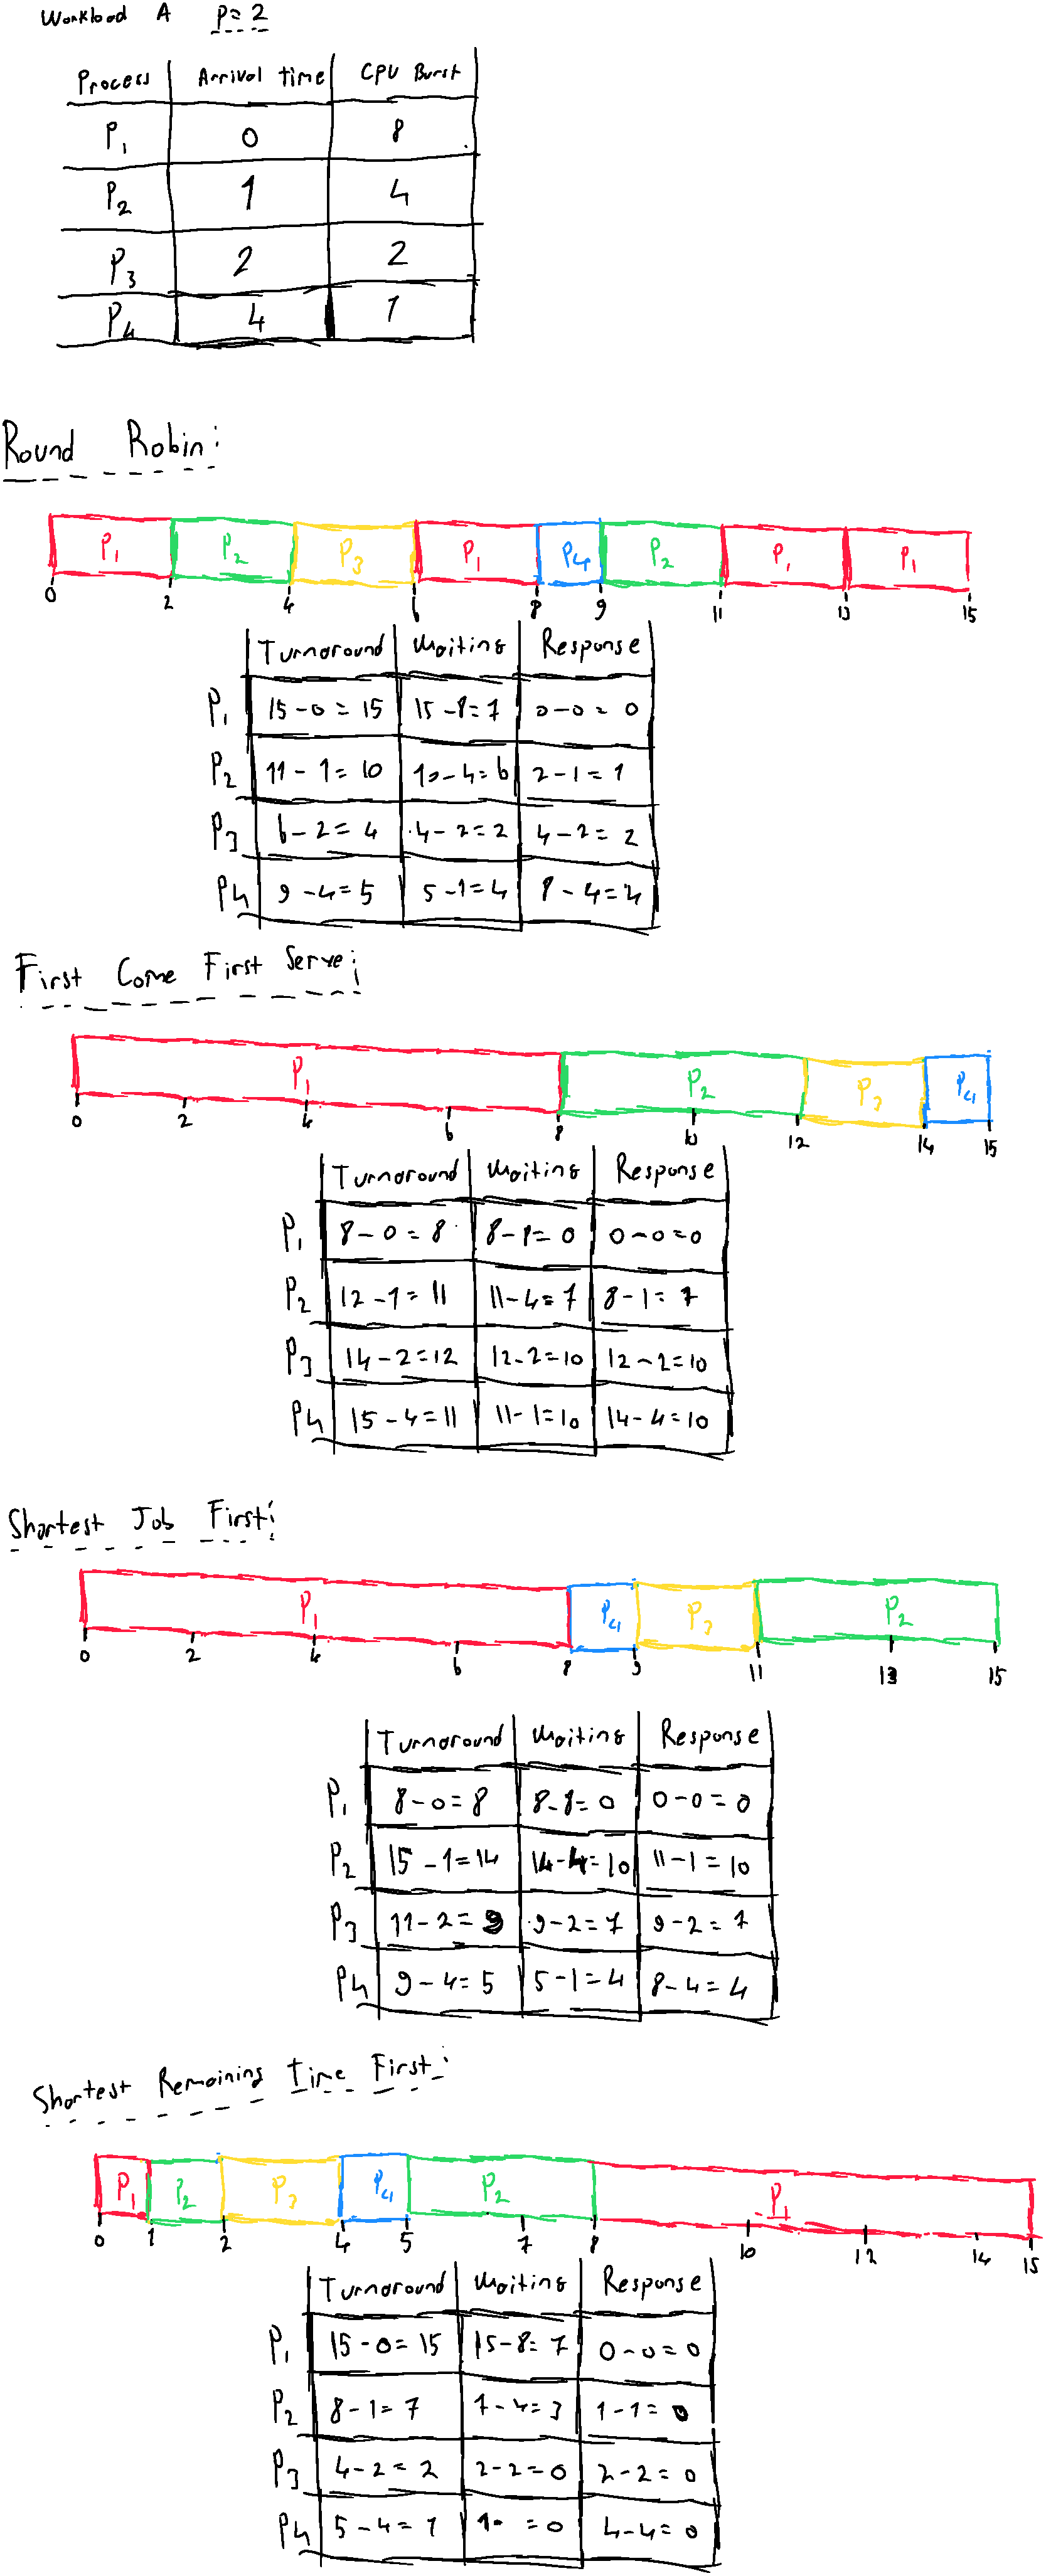
\includegraphics[height=0.86\textheight]{../tests/oracle/Example_Solutions - Workload A.pdf}\hfill
  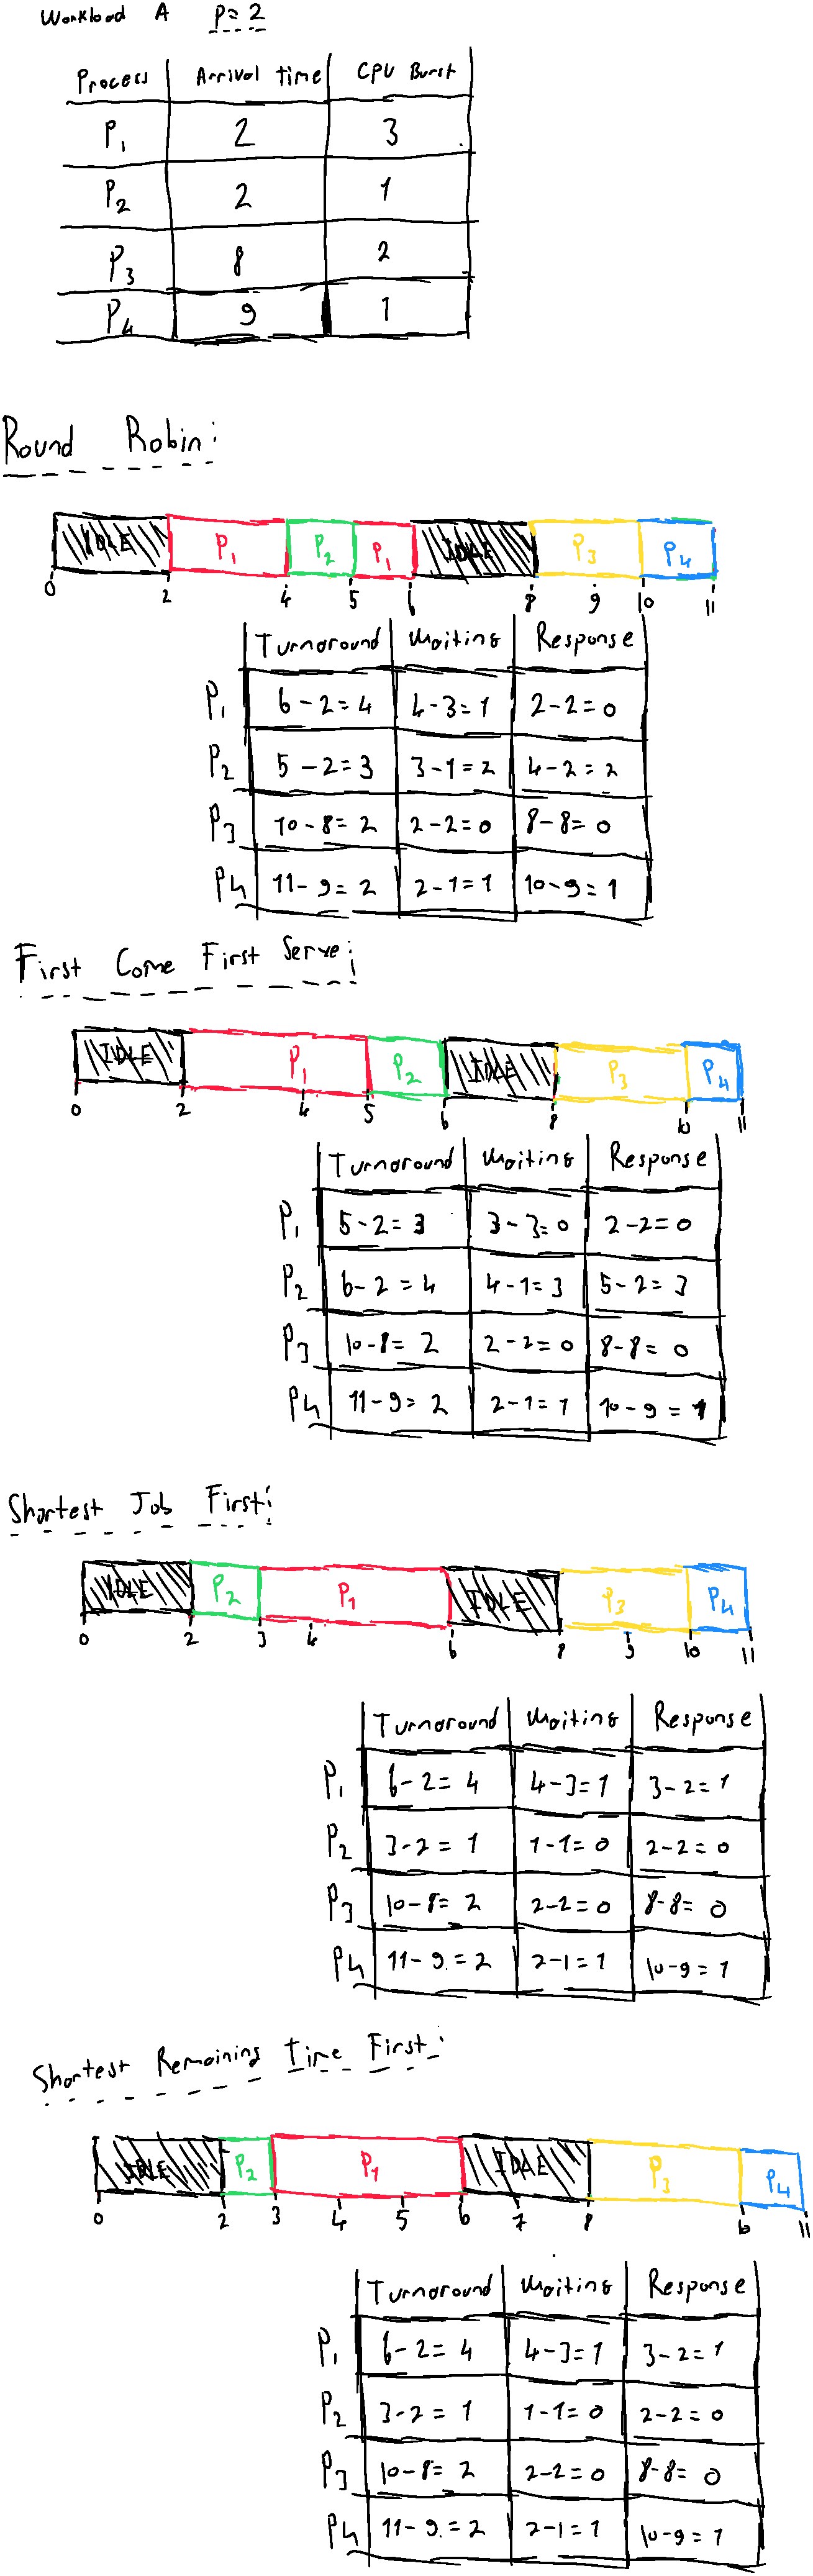
\includegraphics[height=0.86\textheight]{../tests/oracle/Example_Solutions - Workload B.pdf}
\end{center}
\clearpage
\begin{center}
  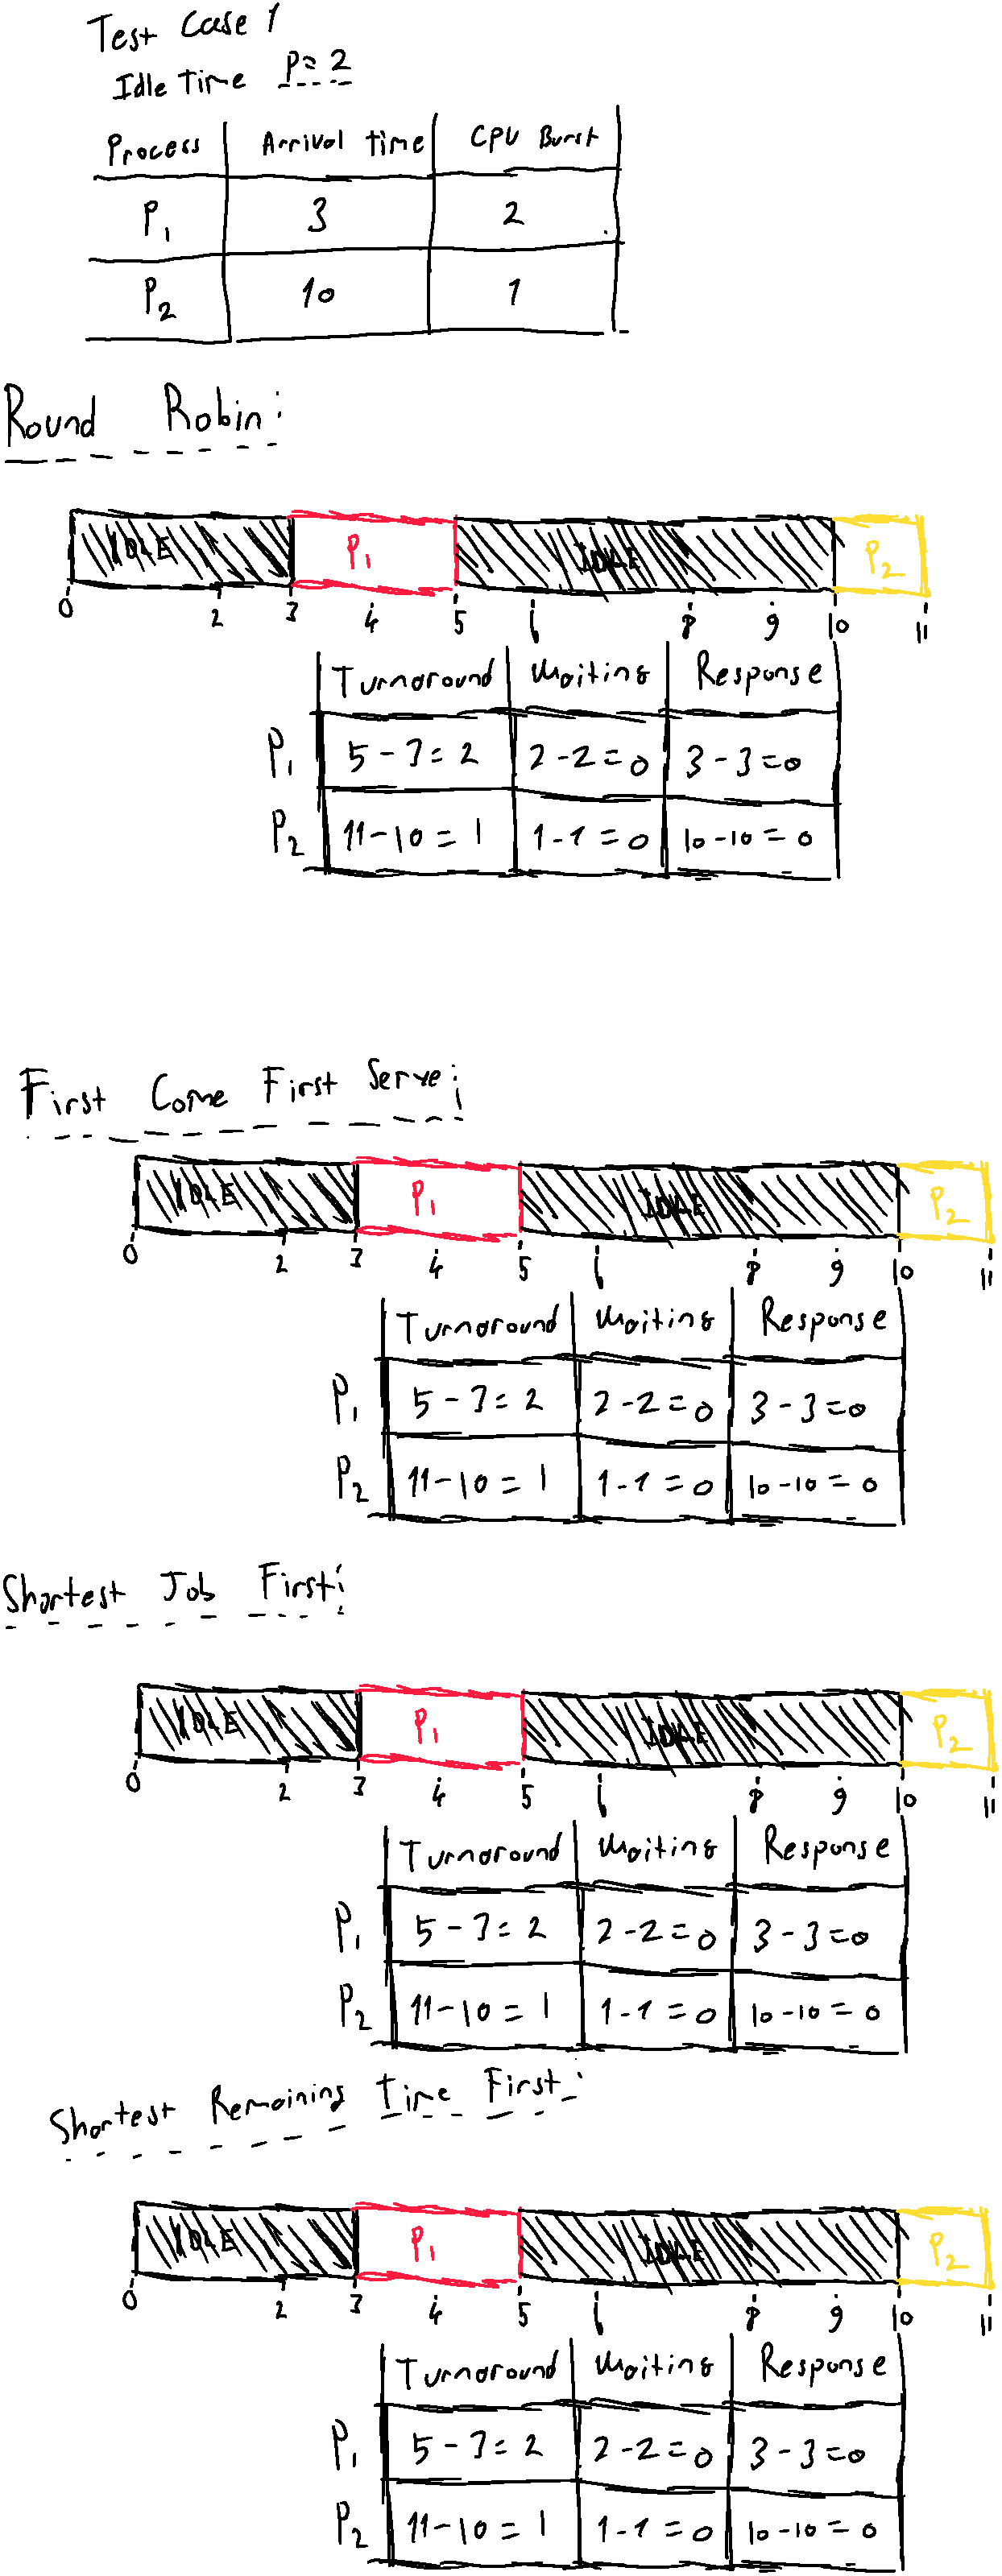
\includegraphics[height=0.86\textheight]{../tests/oracle/Example_Solutions - TC-l.pdf}\hfill
  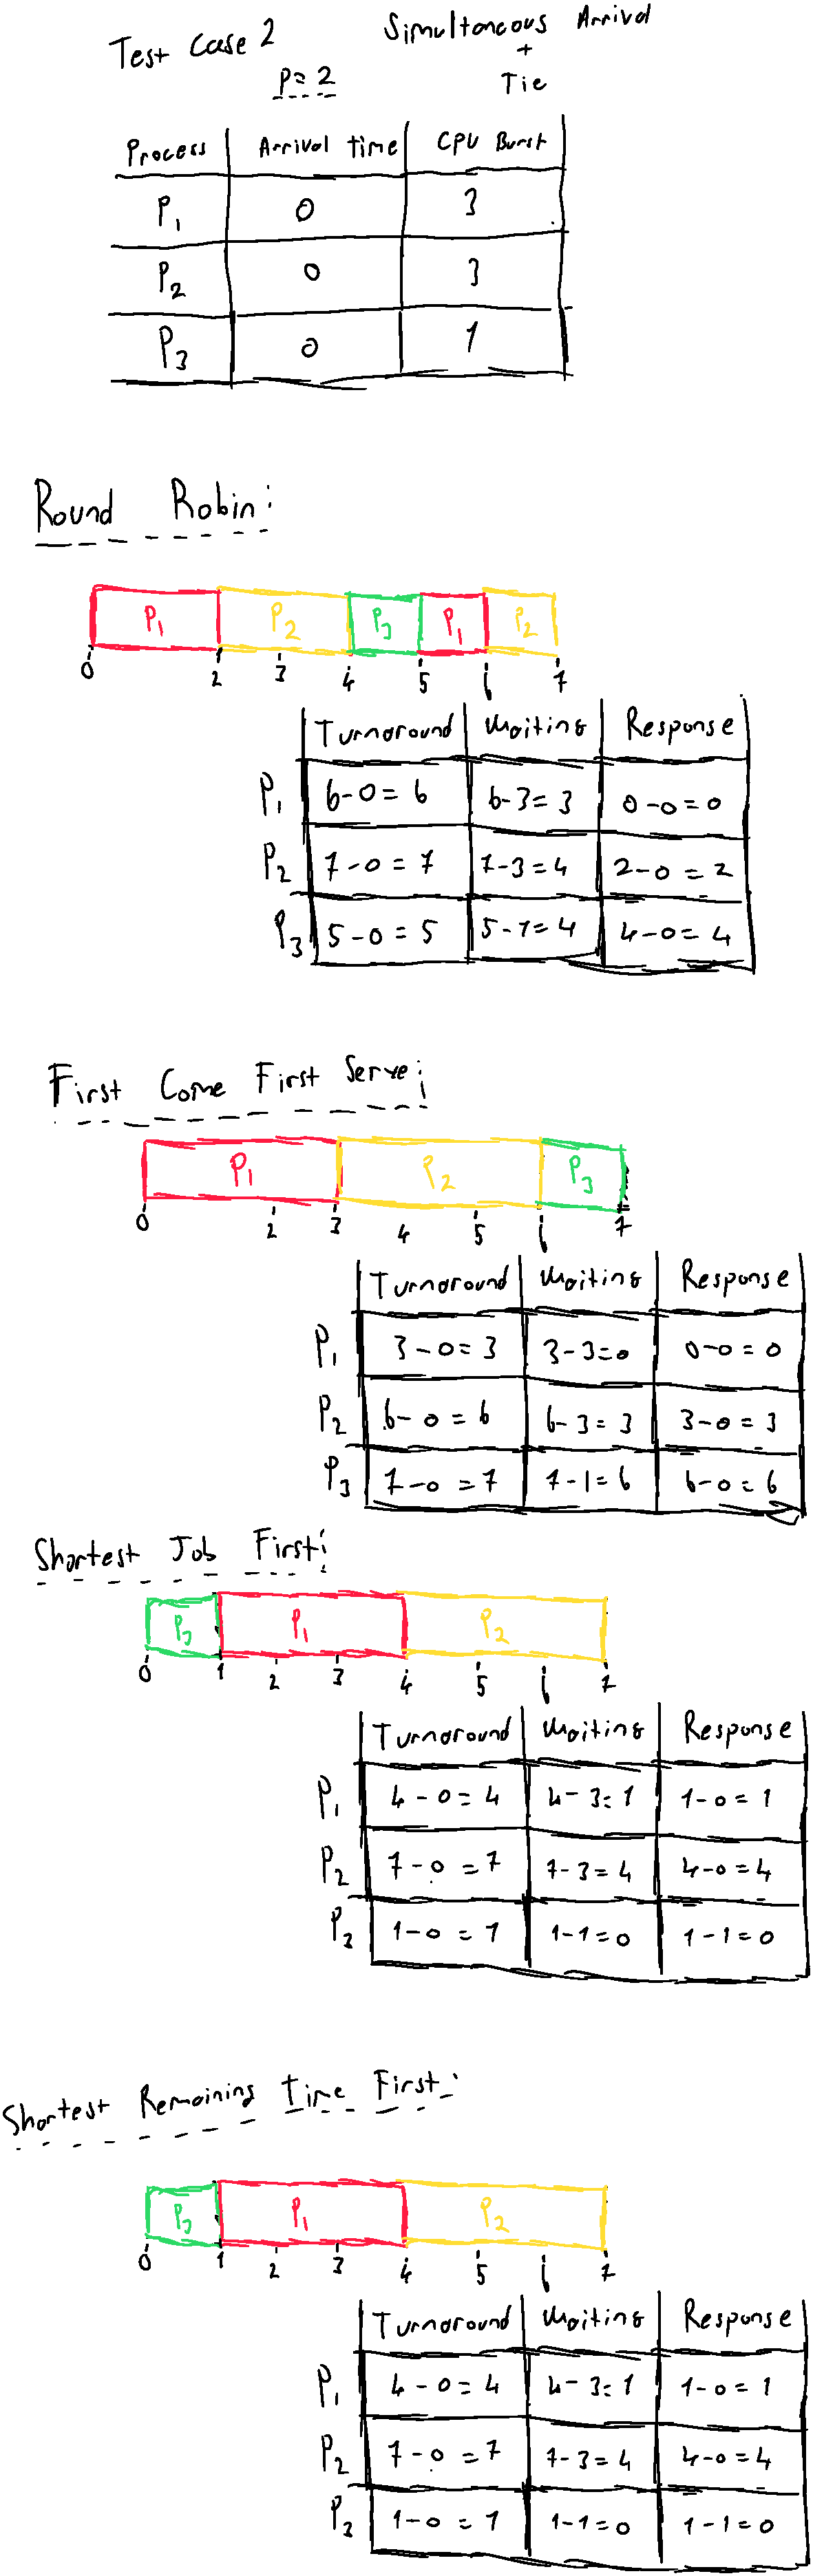
\includegraphics[height=0.86\textheight]{../tests/oracle/Example_Solutions - TC-2.pdf}\hfill
  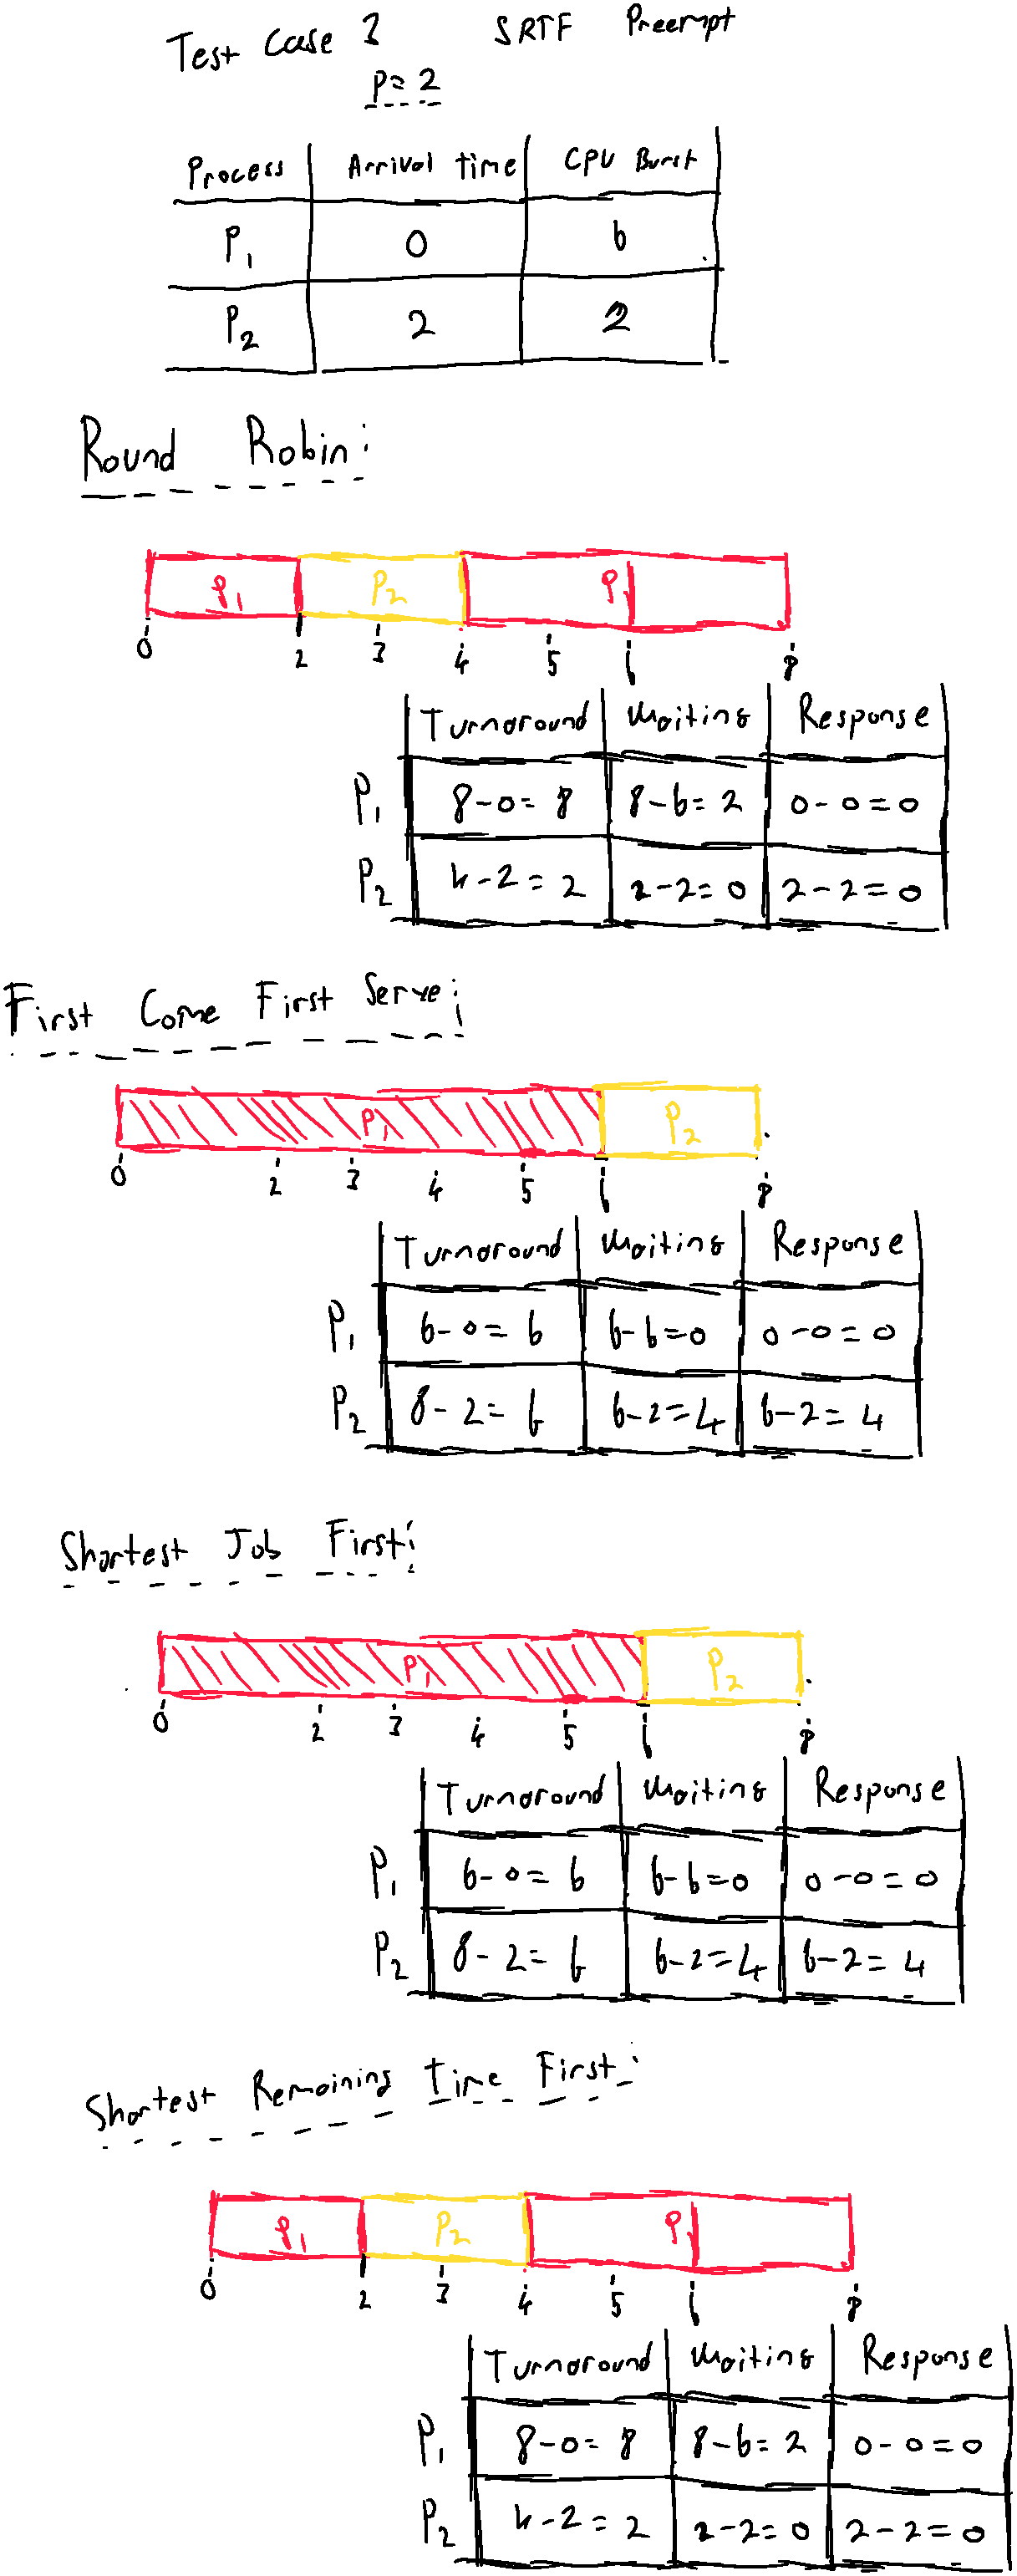
\includegraphics[height=0.86\textheight]{../tests/oracle/Example_Solutions - Tc-3.pdf}
\end{center}

\end{document}
